\mfpicnumber{1}

\opengraphsfile{GraphsofFunctions}

\setcounter{footnote}{0}

\label{GraphsofFunctions}

In Section \ref{IntrotoFunctions} we defined a function as a special type of relation; one in which each $x$-coordinate was matched with only one $y$-coordinate.  We spent most of our time in that section looking at functions graphically because they were, after all, just sets of points in the plane. Then in Section \ref{FunctionNotation} we described a function as a process and defined the notation necessary to work with functions algebraically.  So now it's time to look at functions graphically again, only this time we'll do so with the notation defined in Section \ref{FunctionNotation}.  We start with what should not be a surprising connection.

\medskip

\colorbox{ResultColor}{\bbm

%\smallskip

\centerline{\textbf{The Fundamental Graphing Principle for Functions}}

\label{fgpff} \index{function ! Fundamental Graphing Principle} \index{graph ! of a function} \index{Fundamental Graphing Principle ! for functions}

\smallskip

The graph of a function $f$ is the set of points which satisfy the equation $y=f(x)$.  That is, the point $(x,y)$ is on the graph of $f$ if and only if $y=f(x)$.

\ebm}

\begin{ex}  Graph $f(x) = x^2 - x - 6$.

\medskip

{\bf Solution.}  To graph $f$, we graph the equation $y = f(x)$.  To this end, we use the techniques outlined in Section \ref{GraphsofEquations}.  Specifically, we check for intercepts, test for symmetry, and plot additional points as needed.  To find the $x$-intercepts, we set $y=0$. Since $y = f(x)$, this means $f(x) = 0$. \[ \begin{array}{rclr}   

f(x) & = & x^2 - x - 6 & \\ 
0 & = & x^2 - x - 6 & \\ 
0 & = & (x-3)(x+2) & \mbox{factor} \\ 
x-3 = 0 & \mbox{or} & x+2 = 0 & \\
x & = & -2, 3 & \\

\end{array} \]

So we get $(-2,0)$ and $(3,0)$ as $x$-intercepts.  To find the $y$-intercept, we set $x=0$.  Using function notation, this is the same as finding $f(0)$ and  $f(0) = 0^2 - 0 - 6 = -6.$  Thus the $y$-intercept is $(0,-6)$.  As far as symmetry is concerned, we can tell from the intercepts that the graph possesses none of the three symmetries discussed thus far. (You should verify this.)  We can make a table analogous to the ones we made in Section \ref{GraphsofEquations}, plot the points and connect the dots in a somewhat pleasing fashion to get the graph below on the right.

\hspace{.5in} \begin{tabular}{m{2.7in}m{3in}}

\[ \begin{array}{|r||r|r|}  

\hline

 x & f(x) & (x,f(x)) \\ \hline
-3  & 6 & (-3, 6) \\  \hline
-2  & 0 & (-2,0) \\  \hline
-1 & -4 & ( -1, -4) \\  \hline
0  & -6 & ( 0 ,-6) \\  \hline
1 & -6 & ( 1, -6) \\  \hline
2  & -4 & (2,-4) \\  \hline
3  & 0 & (3, 0) \\  \hline
4  & 6 & (4, 6) \\  \hline
\end{array} \] &

\begin{mfpic}[10]{-4}{5}{-6.5}{7.5}
\point[3pt]{(-3,6), (-2,0), (-1,-4), (0,-6), (1,-6), (2,-4), (3,0), (4,6)}
\axes
\tlabel[cc](5,-0.5){\scriptsize $x$}
\tlabel[cc](0.5,7.5){\scriptsize $y$}
\xmarks{-3,-2,-1,1,2,3,4}
\ymarks{-6,-5,-4,-3,-2,-1,1,2,3,4,5,6,7}
\tlpointsep{4pt}
\axislabels {x}{{\tiny $-3 \hspace{7pt}$} -3, {\tiny $-2 \hspace{7pt}$} -2, {\tiny $-1 \hspace{7pt}$} -1, {\tiny $1$} 1, {\tiny $2$} 2, {\tiny $3$} 3, {\tiny $4$} 4}
\axislabels {y}{{\tiny $-6$} -6,{\tiny $-5$} -5,{\tiny $-4$} -4,{\tiny $-3$} -3,{\tiny $-2$} -2,{\tiny $-1$} -1, {\tiny $1$} 1, {\tiny $2$} 2, {\tiny $3$} 3, {\tiny $4$} 4, {\tiny $5$} 5, {\tiny $6$} 6, {\tiny $7$} 7}
\arrow \reverse \arrow \function{-3.1, 4.1, 0.1}{x**2-x-6}
\end{mfpic} \\

\end{tabular}

\vspace{-.1in}

\qed

\end{ex}

Graphing piecewise-defined functions is a bit more of a challenge.

\begin{ex} Graph:  $f(x) = \left\{ \begin{array}{rcl} 4-x^2 & \mbox{if} &  x < 1 \\ x - 3, & \mbox{if} & x \geq 1 \\ \end{array} \right.$

\medskip

{\bf Solution.}  We proceed as before -- finding intercepts, testing for symmetry and then plotting additional points as needed.  To find the $x$-intercepts, as before, we set $f(x)=0$.  The twist is that we have two formulas for $f(x)$.  For $x<1$, we use the formula $f(x) = 4-x^2$.  Setting $f(x) = 0$ gives $0 = 4 - x^2$, so that $x = \pm 2$.  However, of these two answers, only $x = -2$ fits in the domain $x < 1$ for this piece.  This means the only $x$-intercept for the $x < 1$ region of the $x$-axis is $(-2,0)$.  For $x \geq 1$, $f(x) = x-3$.  Setting $f(x) = 0$ gives  $0 = x-3$,  or $x=3$.  Since $x=3$ satisfies the inequality $x \geq 1$, we get $(3,0)$ as another $x$-intercept.  Next, we seek the $y$-intercept.  Notice that $x=0$ falls in the domain $x < 1$. Thus $f(0) = 4 - 0^2 = 4$ yields the $y$-intercept $(0,4)$.  As far as symmetry is concerned, you can check that the equation $y = 4 - x^2$ is symmetric about the $y$-axis;  unfortunately, this equation (and its symmetry) is valid only for $x < 1$.  You can also verify $y = x - 3$ possesses none of the symmetries discussed in the Section \ref{GraphsofEquations}. When plotting additional points, it is important to keep in mind the restrictions on $x$ for each piece of the function.  The sticking point for this function is $x=1$, since this is where the equations change.  When $x=1$, we use the formula $f(x) = x-3$, so the point on the graph $(1, f(1))$ is $(1,-2)$.  However, for all values less than $1$, we use the formula $f(x) = 4 - x^2$.  As we have discussed earlier in Section \ref{Relations}, there is no real number which immediately precedes $x=1$ on the number line.  Thus for the values $x = 0.9$, $x = 0.99$, $x=0.999$, and so on, we find the corresponding $y$ values using the formula $f(x) = 4 - x^2$.  Making a table as before, we see that as the $x$ values sneak up to $x=1$ in this fashion, the $f(x)$ values inch closer and closer\footnote{We've just stepped into Calculus here!} to $4 - 1^2 = 3$.  To indicate this graphically, we use an open circle at the point $(1,3)$.  Putting all of this information together and plotting additional points, we get

\medskip

\hspace{.5in} \begin{tabular}{m{3in}m{2.7in}}

\[ \begin{array}{|r||c|c|}  \hline

 x & f(x) & (x,f(x)) \\ \hline
0.9  & 3.19 & (0.9, 3.19) \\  \hline
0.99 & \approx 3.02 & (0.99,3.02) \\  \hline
0.999 & \approx 3.002 & ( 0.999, 3.002) \\  \hline

\end{array} \] &

\begin{mfpic}[15]{-4}{4}{-5}{5}
\point[3pt]{(-2,0), (0,4), (1,-2), (3,0)}
\arrow \reverse \function{-3,1,0.1}{4-x**2}
\arrow \function{1,5,0.1}{x-3}
\gclear \circle{(1,3),0.1}
\circle{(1,3),0.1}
\axes
\tlabel[cc](4,-0.5){$x$}
\tlabel[cc](0.5,5){$y$}
\xmarks{-3,-2,-1,1,2,3}
\ymarks{-4,-3,-2,-1,1,2,3,4}
\tlpointsep{5pt}
\scriptsize
\axislabels {x}{{$-3 \hspace{7pt}$} -3, {$-2 \hspace{7pt}$} -2, {$-1 \hspace{7pt}$} -1, {$1$} 1, {$2$} 2, {$3$} 3}
\axislabels {y}{{$-4$} -4,{$-3$} -3,{$-2$} -2,{$-1$} -1, {$1$} 1, {$2$} 2, {$3$} 3, {$4$} 4}
\normalsize
\end{mfpic} \\

\end{tabular}

\qed

\end{ex}

\pagebreak

In the previous two examples, the $x$-coordinates of the $x$-intercepts of the graph of $y=f(x)$ were found by solving $f(x) = 0$.  For this reason, they are called the \index{function ! zero} \textbf{zeros} of $f$.

\smallskip

\colorbox{ResultColor}{\bbm

%\smallskip

\begin{defn}

\label{zerosofafunction} \index{zero ! of a function}

The \textbf{zeros} of a function $f$ are the solutions to the equation $f(x) = 0$.  In other words, $x$ is a zero of $f$ if and only if $(x,0)$ is an $x$-intercept of the graph of $y=f(x)$.

\end{defn}

\ebm}

\medskip

Of the three symmetries discussed in Section \ref{GraphsofEquations}, only two are of significance to functions:  symmetry about the $y$-axis and symmetry about the origin.\footnote{Why are we so dismissive about symmetry about the $x$-axis for graphs of functions?}  Recall that we can test whether the graph of an equation is symmetric about the $y$-axis by replacing $x$ with $-x$ and checking to see if an equivalent equation results.  If we are graphing the equation $y=f(x)$, substituting $-x$ for $x$ results in the equation $y=f(-x)$.  In order for this equation to be equivalent to the original equation $y=f(x)$ we need $f(-x) = f(x)$.  In a similar fashion, we recall that to test an equation's graph for symmetry about the origin, we replace $x$ and $y$ with $-x$ and $-y$, respectively.  Doing this substitution in the equation $y = f(x)$ results in $-y = f(-x)$.  Solving the latter equation for $y$ gives $y = -f(-x)$.  In order for this equation to be equivalent to the original equation $y=f(x)$ we need $-f(-x) = f(x)$, or, equivalently, $f(-x) = -f(x)$.  These results are summarized below.

\medskip

\colorbox{ResultColor}{\bbm

%\smallskip

\centerline{\textbf{Testing the Graph of a Function for Symmetry}}

\smallskip

\hspace{.17in} The graph of a function $f$ is symmetric \index{symmetry ! testing a function graph for}

\begin{itemize}

\item  about the $y$-axis if and only if $f(-x) = f(x)$ for all $x$ in the domain of $f$.

\item  about the origin if and only if $f(-x) = -f(x)$ for all $x$ in the domain of $f$.

\end{itemize}

\ebm}

\medskip

For reasons which won't become clear until we study polynomials, we call a function \index{function ! even}\index{even function}\textbf{even} if its graph is symmetric about the $y$-axis or \index{function ! odd}\index{odd function}\textbf{odd} if its graph is symmetric about the origin.  Apart from a very specialized family of functions which are both even and odd,\footnote{Any ideas?} functions fall into one of three distinct categories: even, odd, or neither even nor odd.  

\begin{ex}  Determine analytically if the following functions are even, odd, or neither even nor odd.  Verify your result with a graphing calculator.

\setlength{\extrarowheight}{2pt}

\begin{multicols}{2}
\begin{enumerate}

\item  $f(x) = \dfrac{5}{2 - x^2}$ 
\item  $g(x) = \dfrac{5x}{2 - x^2}$  

\setcounter{HW}{\value{enumi}}
\end{enumerate}
\end{multicols}

\begin{multicols}{2}
\begin{enumerate}
\setcounter{enumi}{\value{HW}}

\item  $h(x) = \dfrac{5x}{2 - x^3}$
\item  $i(x) = \dfrac{5x}{2x - x^3}$ 

\setcounter{HW}{\value{enumi}}
\end{enumerate}
\end{multicols}

\begin{multicols}{2}
\begin{enumerate}
\setcounter{enumi}{\value{HW}}

\item  $j(x) = x^2 - \dfrac{x}{100}-1$ 
\item  $p(x) = \left\{ \begin{array}{rcl} x+3 & \text{if} &  x < 0 \\ -x+3, & \mbox{if} & x \geq 0 \\ \end{array} \right.$

\setcounter{HW}{\value{enumi}}
\end{enumerate}
\end{multicols}

\medskip

{\bf Solution.} The first step in all of these problems is to replace $x$ with $-x$ and simplify.

\begin{enumerate}

\setlength{\extrarowheight}{8pt}

\item  \[ \begin{array}{rclr}   

f(x) & = & \dfrac{5}{2 - x^2} & \\ 
f(-x) & = & \dfrac{5}{2 - (-x)^2} & \\  
f(-x) & = & \dfrac{5}{2 - x^2} & \\  
f(-x) & = & f(x) & \\

\end{array} \]

Hence, $f$ is \textbf{even}.  The graphing calculator furnishes the following.

\setlength{\extrarowheight}{2pt}

\begin{center}

\begin{tabular}{cc}

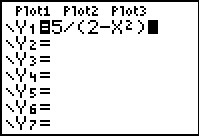
\includegraphics[width=2in]{./RelationsandFunctionsGraphics/GraphsofFunctions01.jpg} \hspace{.75in} & 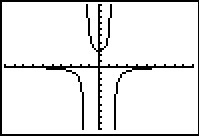
\includegraphics[width=2in]{./RelationsandFunctionsGraphics/GraphsofFunctions02.jpg} \\

\end{tabular}

\end{center}

This suggests\footnote{`Suggests' is about the extent of what it can do.} that the graph of $f$ is symmetric about the $y$-axis, as expected.

\setlength{\extrarowheight}{8pt}

\item  \[ \begin{array}{rclr}   

g(x) & = & \dfrac{5x}{2 - x^2} & \\ 
g(-x) & = & \dfrac{5(-x)}{2 - (-x)^2} & \\  
g(-x) & = & \dfrac{-5x}{2 - x^2} & \\  

\end{array} \]

It doesn't appear that $g(-x)$ is equivalent to $g(x)$.  To prove this, we check with an $x$ value.  After some trial and error, we see that $g(1) = 5$ whereas $g(-1) = -5$.  This proves that $g$ is not even, but it doesn't rule out the possibility that $g$ is odd. (Why not?)  To check if $g$ is odd, we compare $g(-x)$ with $-g(x)$


 \[ \begin{array}{rclr}   

- g(x) & = & - \dfrac{5x}{2 - x^2} & \\ 
& = &  \dfrac{-5x}{2 - x^2} & \\  
-g(x) & = & g(-x) & \\  

\end{array} \]

\setlength{\extrarowheight}{2pt}

Hence, $g$ is odd.  Graphically,

\begin{center}

\begin{tabular}{cc}

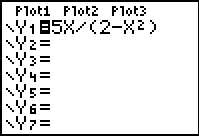
\includegraphics[width=2in]{./RelationsandFunctionsGraphics/GraphsofFunctions03.jpg} \hspace{.75in} & 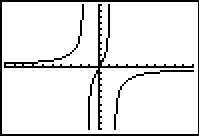
\includegraphics[width=2in]{./RelationsandFunctionsGraphics/GraphsofFunctions04.jpg} \\

\end{tabular}

\end{center}

The calculator indicates the graph of $g$ is symmetric about the origin, as expected.

\setlength{\extrarowheight}{8pt}

\item  \[ \begin{array}{rclr}   

h(x) & = & \dfrac{5x}{2 - x^3} & \\ 
h(-x) & = & \dfrac{5(-x)}{2 - (-x)^3} & \\  
h(-x) & = & \dfrac{-5x}{2 + x^3} & \\  

\end{array} \]

\setlength{\extrarowheight}{2pt}

Once again, $h(-x)$ doesn't appear to be equivalent to $h(x)$.  We check with an $x$ value, for example, $h(1) = 5$ but $h(-1) = -\frac{5}{3}$.  This proves that $h$ is not even and it also shows $h$ is not odd. (Why?)  Graphically,

\begin{center}

\begin{tabular}{cc}

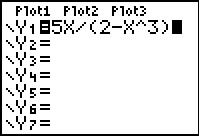
\includegraphics[width=2in]{./RelationsandFunctionsGraphics/GraphsofFunctions05.jpg} \hspace{.75in} & 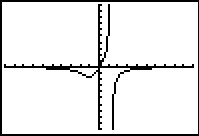
\includegraphics[width=2in]{./RelationsandFunctionsGraphics/GraphsofFunctions06.jpg} \\

\end{tabular}

\end{center}

The graph of $h$ appears to be neither symmetric about the $y$-axis nor the origin.

\setlength{\extrarowheight}{8pt}

\item  \[ \begin{array}{rclr}   

i(x) & = & \dfrac{5x}{2x - x^3} & \\ 
i(-x) & = & \dfrac{5(-x)}{2(-x) - (-x)^3} & \\ 
i(-x) & = & \dfrac{-5x}{-2x + x^3} & \\  

\end{array} \]

\setlength{\extrarowheight}{2pt}

The expression  $i(-x)$ doesn't appear to be equivalent to $i(x)$.  However, after checking some $x$ values, for example $x=1$ yields $i(1) = 5$ and $i(-1 )= 5$, it appears that $i(-x)$ does, in fact, equal $i(x)$.  However, while this suggests  $i$ is even, it doesn't prove it.  (It does, however, prove $i$ is not odd.)  To prove $i(-x) = i(x)$, we need to manipulate our expressions for $i(x)$ and $i(-x)$ and show that they are equivalent.  A clue as to how to proceed is in the numerators: in the formula for $i(x)$, the numerator is $5x$ and in $i(-x)$ the numerator is $-5x$.  To re-write $i(x)$ with a numerator of $-5x$, we need to multiply its numerator by $-1$.  To keep the value of the fraction the same, we need to multiply the denominator by $-1$ as well.  Thus

\setlength{\extrarowheight}{8pt}

 \[ \begin{array}{rclr}   

i(x) & = & \dfrac{5x}{2x - x^3} & \\ 
& = & \dfrac{(-1) 5x}{(-1)\left(2x - x^3\right)} & \\ 
& = & \dfrac{-5x}{-2x + x^3} & \\  

\end{array} \]

\setlength{\extrarowheight}{2pt}

Hence, $i(x) = i(-x)$, so $i$ is even.  The calculator supports our conclusion.

\begin{center}

\begin{tabular}{cc}

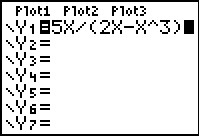
\includegraphics[width=2in]{./RelationsandFunctionsGraphics/GraphsofFunctions07.jpg} \hspace{.75in} & 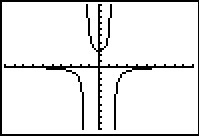
\includegraphics[width=2in]{./RelationsandFunctionsGraphics/GraphsofFunctions08.jpg} \\

\end{tabular}

\end{center}

\setlength{\extrarowheight}{8pt}

\item  \[ \begin{array}{rclr}   

j(x) & = & x^2 - \dfrac{x}{100} - 1 & \\ 
j(-x) & = & (-x)^2 - \dfrac{-x}{100} - 1 & \\   
j(-x) & = & x^2 + \dfrac{x}{100} - 1 & \\   

\end{array} \]

\setlength{\extrarowheight}{2pt}

The expression for $j(-x)$ doesn't seem to be equivalent to $j(x)$, so we check using $x = 1$ to get $j(1) = -\frac{1}{100}$ and $j(-1) = \frac{1}{100}$.  This rules out $j$ being even.  However, it doesn't rule out $j$ being odd.  Examining $-j(x)$ gives

\setlength{\extrarowheight}{8pt}

 \[ \begin{array}{rclr}   

j(x) & = & x^2 - \dfrac{x}{100} - 1 & \\ 
-j(x) & = & -\left(x^2 - \dfrac{x}{100} - 1\right) & \\   
-j(x) & = & -x^2 + \dfrac{x}{100} + 1 & \\   

\end{array} \]

\setlength{\extrarowheight}{2pt}

The expression $-j(x)$ doesn't seem to match $j(-x)$ either.  Testing $x = 2$ gives $j(2) = \frac{149}{50}$ and $j(-2) = \frac{151}{50}$, so $j$ is not odd, either.  The calculator gives:

\begin{center}

\begin{tabular}{cc}

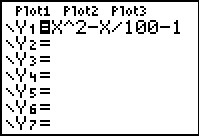
\includegraphics[width=2in]{./RelationsandFunctionsGraphics/GraphsofFunctions09.jpg} \hspace{.75in} & 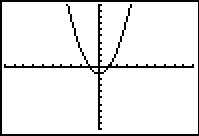
\includegraphics[width=2in]{./RelationsandFunctionsGraphics/GraphsofFunctions10.jpg} \\

\end{tabular}

\end{center}

The calculator suggests that the graph of $j$ is symmetric about the $y$-axis which would imply that $j$ is even. However, we have proven that is not the case.  \qed


\item Testing the graph of $y=p(x)$ for symmetry is complicated by the fact $p(x)$ is a piecewise-defined function.  As always, we handle this by checking the condition for symmetry by checking it on each piece of the domain.  We first consider the case when $x < 0$ and set about finding the correct expression for $p(-x)$.  Even though $p(x) = x+3$ for $x < 0$, $p(-x) \neq -x + 3$ here. The reason for this is that since $x < 0$, $-x > 0$ which means to find $p(-x)$, we need to use the \textit{other} formula for $p(x)$, namely $p(x) = -x+3$. Hence, for $x < 0$, $p(-x) = -(-x)+3 = x+3 = p(x)$.   For $x \geq 0$, $p(x) = -x+3$ and we have two cases.  If $x > 0$, then $-x < 0$ so $p(-x) = (-x)+3 = -x+3 = p(x)$.  If $x = 0$, then $p(0) = 3 = p(-0)$.  Hence, in all cases, $p(-x) = p(x)$, so $p$ is even. Since $p(0) = 3$ but $p(-0) = p(0) = 3 \neq -3$, we also have $p$ is not odd.  While graphing $y=p(x)$ is not onerous to do by hand, it is instructive to see how to enter this into our calculator.  By using some of the logical commands,\footnote{Consult your owner's manual, instructor, or favorite video site!} we have:

\begin{center}

\begin{tabular}{cc}

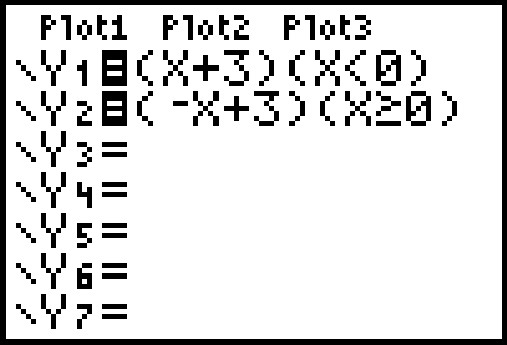
\includegraphics[width=2in]{./RelationsandFunctionsGraphics/PWISE01.jpg} \hspace{.75in} & 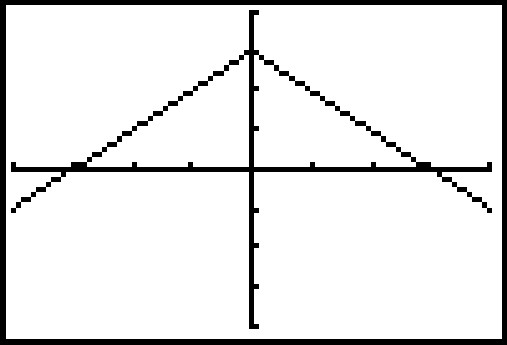
\includegraphics[width=2in]{./RelationsandFunctionsGraphics/PWISE02.jpg} \\

\end{tabular}

\end{center}
 
The calculator bears shows that the graph appears to be symmetric about the $y$-axis. \qed

\end{enumerate}

\end{ex}

There are two lessons to be learned from the last example.  The first is that sampling function values at particular $x$ values is not enough to prove that a function is even or odd $-$ despite the fact that $j(-1) = - j(1)$, $j$ turned out not to be odd.  Secondly, while the calculator may \emph{suggest} mathematical truths, it is the Algebra which \emph{proves} mathematical truths.\footnote{Or, in other words, don't rely too heavily on the machine!}

\medskip

\subsection{General Function Behavior}
\label{genfuncbehavior}

The last topic we wish to address in this section is general function behavior.  As you shall see in the next several chapters, each family of functions has its own unique attributes and we will study them all in great detail.  The purpose of this section's discussion, then, is to lay the foundation for that further study by investigating aspects of function behavior which apply to all functions.  To start, we will examine the concepts of \index{increasing function ! intuitive definition of} {\bf increasing}, \index{decreasing function ! intuitive definition of} {\bf decreasing} and \index{constant function ! intuitive definition of} {\bf constant}.  Before defining the concepts algebraically, it is instructive to first look at them graphically.  Consider the graph of the function $f$ below. 

\begin{center}

\begin{mfpic}[15]{-5}{8}{-10}{8}
\point[3pt]{(-4,-3.1),(-2,4.5), (3,-8), (6.01,5.53), (4.1,-5.91), (5,-5.91)}
\tlabel[cc](-4,-4){\small $(-4,-3)$}
\tlabel[cc](-2.5,5.5){\small $(-2,4.5)$}
\tlabel[cc](3,-9){\small $(3,-8)$}
\tlabel[cc](6.01,6.5){\small $(6,5.5)$}
\tlabel[cc](3,-5){\small $(4,-6)$}
\tlabel[cc](6,-7){\small $(5,-6)$}
\tcaption{The graph of $y=f(x)$}
\function{-4,4.1,0.1}{(2*(x**3)-3*(x**2)-36*x+1)/10}
\function{4.1, 5, 0.1}{-5.91}
\function{5,6.01,0.1}{(2*(x**3)-3*(x**2)-36*x+1)/10-5.51}
\axes
\tlabel[cc](8,-0.5){\scriptsize $x$}
\tlabel[cc](0.5,8){\scriptsize $y$}
\xmarks{-4,-3,-2,-1,1,2,3,4,5,6,7}
\ymarks{-9,-8,-7,-6,-5,-4,-3,-2,-1,1,2,3,4,5,6,7}
\tlpointsep{5pt}
\scriptsize
\axislabels {x}{{$-4 \hspace{7pt}$} -4, {$-3 \hspace{7pt}$} -3, {$-2 \hspace{7pt}$} -2, {$-1 \hspace{7pt}$} -1, {$1$} 1, {$2$} 2, {$3$} 3,  {$4$} 4, {$5$} 5, {$6$} 6, {$7$} 7}
\axislabels {y}{ {$-9$} -9,{$-8$} -8,{$-7$} -7, {$-6$} -6,{$-5$} -5,{$-4$} -4, {$-3$} -3,{$-2$} -2,{$-1$} -1,{$1$} 1, {$2$} 2, {$3$} 3 ,{$1$} 1, {$2$} 2, {$3$} 3 ,{$4$} 4, {$5$} 5, {$6$} 6 ,{$7$} 7}
\normalsize
\end{mfpic}

\end{center}

Reading from left to right, the graph `starts' at the point $(-4,-3)$ and `ends' at the point $(6,5.5)$.  If we imagine walking from left to right on the graph, between $(-4,-3)$ and $(-2,4.5)$, we are walking `uphill'; then between $(-2,4.5)$ and $(3,-8)$, we are walking `downhill'; and between $(3,-8)$ and $(4,-6)$, we are walking `uphill' once more.  From $(4,-6)$ to $(5, -6)$, we `level off', and then resume walking `uphill' from $(5,-6)$ to $(6,5.5)$.  In other words, for the $x$ values between $-4$ and $-2$ (inclusive), the $y$-coordinates on the graph are getting larger, or \index{function ! increasing} \textbf{increasing}, as we move from left to right.  Since $y = f(x)$, the $y$ values on the graph are the function values, and we say that the function $f$ is \textbf{increasing} on the interval $[-4,-2]$.  Analogously, we say that $f$ is \index{function ! decreasing} \textbf{decreasing} on the interval $[-2,3]$ increasing once more on the interval $[3,4]$, \index{function ! constant} \textbf{constant} on $[4,5]$, and finally increasing once again on $[5,6]$.  It is extremely important to notice that the behavior (increasing, decreasing or constant) occurs on an interval on the $x$-axis.  When we say that the function $f$ is increasing on $[-4, -2]$ we do not mention the actual $y$ values that $f$ attains along the way.  Thus, we report \emph{where} the behavior occurs, not to what extent the behavior occurs.\footnote{The notions of how quickly or how slowly a function increases or decreases are explored in Calculus.}  Also notice that we do not say that a function is increasing, decreasing or constant at a single $x$ value.  In fact, we would run into serious trouble in our previous example if we tried to do so because $x = -2$ is contained in an interval on which $f$ was increasing and one on which it is decreasing.  (There's more on this issue -- and many others -- in the Exercises.) 

\smallskip 

We're now ready for the more formal algebraic definitions of what it means for a function to be increasing, decreasing or constant.

\smallskip

\colorbox{ResultColor}{\bbm

%\smallskip

\begin{defn}

\label{incdeccnstdefn}

Suppose $f$ is a function defined on an interval $I$.  We say $f$ is:

\begin{itemize}

\item \index{increasing function ! formal definition of} \textbf{increasing} on $I$ if and only if $f(a) < f(b)$ for all real numbers $a$, $b$ in $I$ with $a < b$.

\item \index{decreasing function ! formal definition of} \textbf{decreasing} on $I$ if and only if $f(a) > f(b)$ for all real numbers $a$, $b$ in $I$ with $a < b$.

\item \index{constant function ! formal definition of} \textbf{constant} on $I$ if and only if $f(a) = f(b)$ for all real numbers $a$, $b$ in $I$.

\end{itemize}

\end{defn}

\ebm}

\medskip

It is worth taking some time to see that the algebraic descriptions of increasing, decreasing and constant as stated in Definition \ref{incdeccnstdefn} agree with our graphical descriptions given earlier.  You should look back through the examples and exercise sets in previous sections where graphs were given to see if you can determine the intervals on which the functions are increasing, decreasing or constant.  Can you find an example of a function for which none of the concepts in Definition \ref{incdeccnstdefn} apply?

\bigskip

Now let's turn our attention to a few of the points on the graph.  Clearly the point $(-2, 4.5)$ does not have the largest $y$ value of all of the points on the graph of $f\; -$ indeed that honor goes to $(6, 5.5)\; -$ but $(-2, 4.5)$ should get some sort of consolation prize for being `the top of the hill' between $x = -4$ and $x = 3$.  We say that the function $f$ has a \index{function ! local (relative) maximum}\index{local maximum ! intuitive definition of}\textbf{local maximum}\footnote{Also called `relative maximum'.} at the point $(-2,4.5)$, because the $y$-coordinate $4.5$ is the largest $y$-value (hence, function value) on the curve `near'\footnote{We will make this more precise in a moment.} $x=-2$.  Similarly, we say that the function $f$ has a \index{function ! local (relative) minimum}\index{local minimum ! intuitive definition of}\textbf{local minimum}\footnote{Also called a `relative minimum'.} at the point $(3,-8)$, since the $y$-coordinate $-8$ is the smallest function value near $x=3$.  Although it is tempting to say that local extrema\footnote{`Maxima' is the plural of `maximum' and `mimima' is the plural of `minimum'.  `Extrema' is the plural of `extremum' which combines maximum and minimum.} occur when the function changes from increasing to decreasing or vice versa, it is not a precise enough way to define the concepts for the needs of Calculus.  At the risk of being pedantic, we will present the traditional definitions and thoroughly vet the pathologies they induce in the Exercises. We have one last observation to make before we proceed to the algebraic definitions and look at a fairly tame, yet helpful, example.

\smallskip

If we look at the entire graph, we see that the largest $y$ value (the largest function value) is $5.5$ at $x=6$.  In this case, we say the \index{function ! (absolute) maximum}\index{maximum ! intuitive definition of}\textbf{maximum}\footnote{Sometimes called the `absolute' or `global' maximum.} of $f$ is $5.5$;  similarly, the \index{function ! (absolute, global) minimum}\index{minimum ! intuitive definition of}\textbf{minimum}\footnote{Again, `absolute' or `global' minimum can be used.} of $f$ is~$-8$.  

We formalize these concepts in the following definitions.

\medskip

\colorbox{ResultColor}{\bbm

%\smallskip

\begin{defn}

\label{maxmindefn}

Suppose $f$ is a function with $f(a) = b$.

\begin{itemize}

\item  We say $f$ has a \textbf{local maximum} at the point $(a,b)$ if and only if there is an open interval $I$ containing $a$ for which $f(a) \geq f(x)$ for all $x$ in $I$.  The value $f(a) = b$ is called `a  local maximum value of $f$' in this case. \index{local maximum ! formal definition of}
 
\item  We say $f$ has a \textbf{local minimum} at the point $(a,b)$ if and only if there is an open interval $I$ containing $a$ for which $f(a) \leq f(x)$ for all $x$ in $I$.  The value $f(a) = b$ is called `a  local minimum value of $f$' in this case. \index{local minimum ! formal definition of}

\item  The value $b$ is called the \textbf{maximum} of $f$ if $b \geq f(x)$ for all $x$ in the domain of $f$. \index{maximum ! formal definition of}

\item  The value $b$ is called the \textbf{minimum} of $f$ if $b \leq f(x)$ for all $x$ in the domain of $f$. \index{minimum ! formal definition of}

\end{itemize}

\end{defn}

\ebm}

\medskip

It's important to note that not every function will have all of these features.  Indeed, it is possible to have a function with no local or absolute extrema at all!  (Any ideas of what such a function's graph would have to look like?)  We shall see examples of functions in the Exercises which have one or two, but not all, of these features, some that have instances of each type of extremum and some functions that seem to defy common sense.  In all cases, though, we shall adhere to the algebraic definitions above as we explore the wonderful diversity of graphs that functions provide us.

\medskip

Here is the `tame' example which was promised earlier.  It summarizes all of the concepts presented in this section as well as some from previous sections so you should spend some time thinking deeply about it before proceeding to the Exercises.

\begin{ex}  Given the graph of $y = f(x)$ below, answer all of the following questions.
\label{tame}

\begin{center}

\begin{mfpic}[20]{-5}{5}{-5}{5}
\point[3pt]{(-2,0), (2,0), (4,-3), (-4,-3), (0,3)}
\function{-4,4,.1}{3*cos(3.14159265*x/4)}
\tlabel[cc](-3,0.5){\small $\left( -2, 0 \right)$}
\tlabel[cc](2.5,0.5){\small $\left(2, 0 \right)$}
\tlabel[cc](4,-3.5){\small $\left( 4, -3 \right)$}
\tlabel[cc](-4,-3.5){\small $\left(-4, -3 \right)$}
\tlabel[cc](1,3.5){\small $\left(0, 3 \right)$}
\axes
\tlabel[cc](5,-0.5){\scriptsize $x$}
\tlabel[cc](0.5,5){\scriptsize $y$}
\xmarks{-4,-3,-2,-1,1,2,3,4}
\ymarks{-4,-3,-2,-1,1,2,3,4}
\tlpointsep{5pt}
\scriptsize
\axislabels {x}{{$-4 \hspace{7pt}$} -4, {$-3 \hspace{7pt}$} -3, {$-2 \hspace{7pt}$} -2, {$-1 \hspace{7pt}$} -1, {$1$} 1, {$2$} 2, {$3$} 3, {$4$} 4}
\axislabels {y}{{$-4$} -4, {$-3$} -3, {$-2$} -2, {$-1$} -1, {$1$} 1, {$2$} 2, {$3$} 3, {$4$} 4}
\normalsize
\end{mfpic}

\end{center}

\begin{multicols}{2}
\begin{enumerate}

\item  Find the domain of $f$.

\item  Find the range of $f$.

\setcounter{HW}{\value{enumi}}
\end{enumerate}
\end{multicols}

\begin{multicols}{2}
\begin{enumerate}
\setcounter{enumi}{\value{HW}}

\item  List the $x$-intercepts, if any exist.

\item  List the $y$-intercepts, if any exist.

\setcounter{HW}{\value{enumi}}
\end{enumerate}
\end{multicols}

\begin{multicols}{2}
\begin{enumerate}
\setcounter{enumi}{\value{HW}}

\item  Find the zeros of $f$.

\item  Solve $f(x) < 0$.

\setcounter{HW}{\value{enumi}}
\end{enumerate}
\end{multicols}

\begin{multicols}{2}
\begin{enumerate}
\setcounter{enumi}{\value{HW}}

\item  Determine $f(2)$.

\item  Solve $f(x) = -3$.  

\setcounter{HW}{\value{enumi}}
\end{enumerate}
\end{multicols}


\begin{multicols}{2}
\begin{enumerate}
\setcounter{enumi}{\value{HW}}

\item  Find the number of solutions to $f(x) = 1$.

\item  Does $f$ appear to be even, odd, or neither?

\setcounter{HW}{\value{enumi}}
\end{enumerate}
\end{multicols}


\begin{multicols}{2}
\begin{enumerate}
\setcounter{enumi}{\value{HW}}

\item  List the intervals on which $f$ is increasing.

\item  List the intervals on which $f$ is decreasing.

\setcounter{HW}{\value{enumi}}
\end{enumerate}
\end{multicols}

\begin{multicols}{2}
\begin{enumerate}
\setcounter{enumi}{\value{HW}}

\item  List the local maximums, if any exist.

\item  List the local minimums, if any exist.

\setcounter{HW}{\value{enumi}}
\end{enumerate}
\end{multicols}

\begin{multicols}{2}
\begin{enumerate}
\setcounter{enumi}{\value{HW}}

\item  Find the maximum, if it exists.

\item  Find the minimum, if it exists.

\setcounter{HW}{\value{enumi}}
\end{enumerate}
\end{multicols}

\medskip

{\bf Solution.} 

\begin{enumerate}

\item  To find the domain of $f$, we proceed as in Section \ref{IntrotoFunctions}.  By projecting the graph to the $x$-axis, we see that the portion of the $x$-axis which corresponds to a point on the graph is everything from $-4$ to $4$, inclusive.  Hence, the domain is $[-4,4]$.

\item  To find the range, we project the graph to the $y$-axis.  We see that the $y$ values from $-3$ to $3$, inclusive, constitute the range of $f$.  Hence, our answer is $[-3,3]$.

\item  The $x$-intercepts are the points on the graph with $y$-coordinate $0$, namely $(-2,0)$ and $(2,0)$.

\item  The $y$-intercept is the point on the graph with $x$-coordinate $0$, namely $(0,3)$.

\item  The zeros of $f$ are the $x$-coordinates of the $x$-intercepts of the graph of $y=f(x)$ which are $x=-2, 2$.

\item  To solve $f(x) < 0$, we look for the $x$ values of the points on the graph where the $y$-coordinate is less than $0$.  Graphically, we are looking for where the graph is below the $x$-axis.  This happens for the $x$ values from $-4$ to $-2$ and again from $2$ to $4$.  So our answer is $[-4,-2) \cup (2,4]$.

\item  Since the graph of $f$ is the graph of the equation $y=f(x)$, $f(2)$ is the $y$-coordinate of the point which corresponds to $x = 2$.  Since the point $(2,0)$ is on the graph, we have $f(2) = 0$.

\item  To solve $f(x) = -3$, we look where $y = f(x) = -3$.  We find two points with a $y$-coordinate of $-3$, namely $(-4,-3)$ and $(4,-3)$.  Hence, the solutions to $f(x) = -3$ are $x = \pm 4$.



\item As in the previous problem, to solve $f(x)=1$, we look for points on the graph where the $y$-coordinate is $1$.  Even though these points aren't specified, we see that the curve has two points with a $y$ value of $1$, as seen in the graph below.  That means there are two solutions to $f(x) = 1$.


\begin{center}

\begin{mfpic}[20]{-5}{5}{-5}{5}
\function{-4,4,.1}{3*cos(3.14159265*x/4)}
\dashed \arrow \reverse \arrow \polyline{(-4,1), (4,1)}
\point[3pt]{(-1.5673,1),(1.5673,1), (-4,-3), (4,-3)}
\axes
\tlabel[cc](5,-0.5){\scriptsize $x$}
\tlabel[cc](0.5,5){\scriptsize $y$}
\xmarks{-4,-3,-2,-1,1,2,3,4}
\ymarks{-4,-3,-2,-1,1,2,3,4}
\tlpointsep{5pt}
\scriptsize
\axislabels {x}{{$-4 \hspace{7pt}$} -4, {$-3 \hspace{7pt}$} -3, {$-2 \hspace{7pt}$} -2, {$-1 \hspace{7pt}$} -1, {$1$} 1, {$2$} 2, {$3$} 3, {$4$} 4}
\axislabels {y}{{$-4$} -4, {$-3$} -3, {$-2$} -2, {$-1$} -1, {$1$} 1, {$2$} 2, {$3$} 3, {$4$} 4}
\normalsize
\end{mfpic}

\end{center}

\vspace{-.1in}

\item  The graph appears to be symmetric about the $y$-axis.  This suggests\footnote{but does not prove} that $f$ is even.

\item  As we move from left to right, the graph rises from $(-4,-3)$ to $(0,3)$.  This means $f$ is increasing on the interval $[-4,0]$.  (Remember, the answer here is an interval on the $x$-axis.)

\item  As we move from left to right, the graph falls from $(0,3)$ to $(4,-3)$.  This means $f$ is decreasing on the interval $[0,4]$.  (Remember, the answer here is an interval on the $x$-axis.)

\item  The function has its only local maximum at $(0,3)$ so $f(0) = 3$ is the local minimum value.

\item  There are no local minimums.  Why don't $(-4, -3)$ and $(4, -3)$ count?  Let's consider the point $(-4, -3)$ for a moment.  Recall that, in the definition of local minimum, there needs to be an open interval $I$ which contains $x = -4$ such that $f(-4) < f(x)$ for all $x$ in $I$ different from $-4$.  But if we put an open interval around $x= -4$ a portion of that interval will lie outside of the domain of $f$.  Because we are unable to fulfill the requirements of the definition for a local minimum, we cannot claim that $f$ has one at $(-4, -3)$.  The point $(4, -3)$ fails for the same reason $-$ no open interval around $x = 4$ stays within the domain of $f$.

\item  The maximum value of $f$ is the largest $y$-coordinate which is $3$.

\item  The minimum value of $f$ is the smallest $y$-coordinate which is $-3$.

\end{enumerate}

\end{ex} 

\vspace{-.32in} \qed

\smallskip

With few exceptions, we will not develop techniques in College Algebra which allow us to determine the intervals on which a function is increasing, decreasing or constant or to find the local maximums and local minimums analytically;  this is the business of Calculus.\footnote{Although, truth be told, there is only one step of Calculus involved, followed by several pages of algebra.}  When we have need to find such beasts, we will resort to the calculator.  Most graphing calculators have `Minimum' and `Maximum' features which can be used to approximate these values, as we now demonstrate.

\begin{ex}  Let $f(x) = \dfrac{15x}{x^2+3}$.  Use a graphing calculator to approximate the intervals on which $f$ is increasing and those on which it is decreasing.  Approximate all extrema.

\medskip

{\bf Solution.}  Entering this function into the calculator gives

\begin{center}

\begin{tabular}{cc}

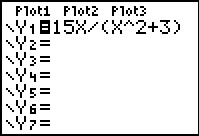
\includegraphics[width=2in]{./RelationsandFunctionsGraphics/GraphsofFunctions11.jpg} \hspace{.75in} & 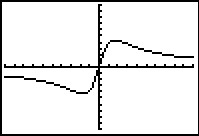
\includegraphics[width=2in]{./RelationsandFunctionsGraphics/GraphsofFunctions12.jpg} \\

\end{tabular}

\end{center}

Using the Minimum and Maximum features, we get

\begin{center}

\begin{tabular}{cc}

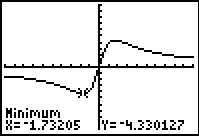
\includegraphics[width=2in]{./RelationsandFunctionsGraphics/GraphsofFunctions13.jpg} \hspace{.75in} & 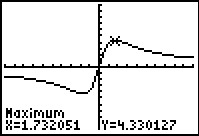
\includegraphics[width=2in]{./RelationsandFunctionsGraphics/GraphsofFunctions14.jpg} \\

\end{tabular}

\end{center}

To two decimal places, $f$ appears to have its only local minimum at $(-1.73, -4.33)$ and its only local maximum at  $(1.73, 4.33)$.  Given the symmetry about the origin suggested by the graph, the relation between these points shouldn't be too surprising.  The function appears to be increasing on $[-1.73, 1.73]$ and decreasing on $(-\infty, -1.73] \cup [1.73,\infty)$.  This makes $-4.33$ the (absolute) minimum and $4.33$ the (absolute) maximum.  \qed


\end{ex}

\begin{ex} \label{distancefunctionex} Find the points on the graph of $y = (x-3)^2$ which are closest to the origin.  Round your answers to two decimal places.

\medskip

{\bf Solution.}  Suppose a point $(x,y)$ is on the graph of $y = (x-3)^2$.  Its distance to the origin $(0,0)$ is given by
 
\setlength{\extrarowheight}{8pt}

\[ \begin{array}{rclr} 

d & = &  \sqrt{(x-0)^2+(y-0)^2} & \\
& = &  \sqrt{x^2+y^2} &  \\
&= & \sqrt{x^2 + \left[(x-3)^2\right]^2} & \mbox{Since $y = (x-3)^2$} \\
& = & \sqrt{x^2 + (x-3)^4} & 

\end{array} \]

\setlength{\extrarowheight}{2pt}

Given a value for $x$, the formula $d =  \sqrt{x^2 + (x-3)^4} $ is the distance from $(0,0)$ to the point $(x,y)$ on the curve $y = (x-3)^2$.  What we have defined, then, is a function $d(x)$ which we wish to minimize over all values of $x$.  To accomplish this task analytically would require Calculus so as we've mentioned before, we can use a graphing calculator to find an approximate solution.   Using the calculator, we enter the function $d(x)$ as shown below and graph.

\begin{center}

\begin{tabular}{cc}

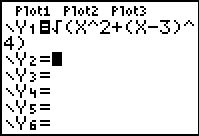
\includegraphics[width=2in]{./RelationsandFunctionsGraphics/YEQU1.jpg} \hspace{.75in} &
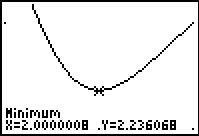
\includegraphics[width=2in]{./RelationsandFunctionsGraphics/DISTBOX1.jpg} \\

\end{tabular}

\end{center}

Using the Minimum feature, we see above on the right that the (absolute) minimum occurs near $x=2$.  Rounding to two decimal places, we get that the minimum distance occurs when $x = 2.00$.  To find the $y$ value on the parabola associated with $x = 2.00$, we substitute $2.00$ into the equation to get $y = (x-3)^2 = (2.00-3)^2 = 1.00$.  So, our final answer is $(2.00,1.00).$\footnote{It seems silly to list a final answer as $(2.00, 1.00)$.  Indeed, Calculus confirms that the \emph{exact} answer to this problem is, in fact, $(2,1)$.  As you are well aware by now, the authors are overly pedantic, and as such, use the decimal places to remind the reader that \emph{any} result garnered from a calculator in this fashion is an approximation, and should be treated as such.}  (What does the $y$ value listed on the calculator screen mean in this problem?)  \qed

\end{ex}

\newpage

\subsection{Exercises}
\label{GraphsofFunctionsExercises}

In Exercises \ref{sketchgraphfirst} - \ref{sketchgraphlast}, sketch the graph of the given function.  State the domain of the function, identify any intercepts and test for symmetry.

\begin{multicols}{3}
\begin{enumerate}

\item $f(x) = 2-x$ \label{sketchgraphfirst}
\item $f(x) = \dfrac{x - 2}{3}$
\item $f(x) = x^2 + 1$

\setcounter{HW}{\value{enumi}}
\end{enumerate}
\end{multicols}

\begin{multicols}{3}
\begin{enumerate}
\setcounter{enumi}{\value{HW}}

\item $f(x) = 4-x^2$
\item $f(x) = 2$
\item $f(x) = x^3$

\setcounter{HW}{\value{enumi}}
\end{enumerate}
\end{multicols}

\begin{multicols}{3}
\begin{enumerate}
\setcounter{enumi}{\value{HW}}

\item $f(x) = x(x-1)(x+2)$
\item $f(x) = \sqrt{x-2}$
\item $f(x) = \sqrt{5 - x}$

\setcounter{HW}{\value{enumi}}
\end{enumerate}
\end{multicols}

\begin{multicols}{3}
\begin{enumerate}
\setcounter{enumi}{\value{HW}}

\item $f(x) = 3-2\sqrt{x+2}$
\item $f(x) = \sqrt[3]{x}$
\item $f(x) = \dfrac{1}{x^{2} + 1}$ \label{sketchgraphlast}

\setcounter{HW}{\value{enumi}}
\end{enumerate}
\end{multicols}

In Exercises \ref{sketchpiecefirst} - \ref{sketchpiecelast}, sketch the graph of the given piecewise-defined function.

\begin{multicols}{2}
\begin{enumerate}
\setcounter{enumi}{\value{HW}}

\item ${\displaystyle f(x) = \left\{ \begin{array}{rcl} 4-x & \mbox{ if } &  x \leq 3 \\
                                                            2 & \mbox{ if } & x > 3 
                                     \end{array} \right. }$ \label{sketchpiecefirst}

\item ${\displaystyle f(x) = \left\{ \begin{array}{rcl} x^2 & \mbox{ if } & x \leq 0 \\
                                                     2x & \mbox{ if } & x > 0
                                  \end{array} \right. }$

\setcounter{HW}{\value{enumi}}
\end{enumerate}
\end{multicols}


\begin{multicols}{2}
\begin{enumerate}
\setcounter{enumi}{\value{HW}}

\item ${\displaystyle f(x) = \left\{ \begin{array}{rcl}  -3 & \mbox{ if } & x < 0 \\
                                                        2x-3 & \mbox{ if } & 0 \leq x \leq 3 \\
                                                            3 & \mbox{ if } & x > 3  
                                     \end{array} \right. }$

\item ${\displaystyle f(x) = \left\{ \begin{array}{rcl} x^2 - 4 & \mbox{ if } &x \leq -2\\
                                                                  4-x^2 & \mbox{ if } & -2 < x < 2 \\
                                                         x^2-4 & \mbox{ if } & x \geq 2 
                                     \end{array} \right. }$


\setcounter{HW}{\value{enumi}}
\end{enumerate}
\end{multicols}


\begin{multicols}{2}
\begin{enumerate}
\setcounter{enumi}{\value{HW}}

\item ${\displaystyle f(x) = \left\{ \begin{array}{rcl} -2x - 4 & \mbox{ if } &  x < 0 \\
                                                             3x & \mbox{ if } & x \geq 0 
                                     \end{array} \right. }$

\item ${\displaystyle f(x) = \left\{ \begin{array}{rcl} \sqrt{x + 4} & \mbox{ if } & -4 \leq x < 5 \\
                                                        \sqrt{x - 1} & \mbox{ if } & x \geq 5
                                     \end{array} \right. }$

\setcounter{HW}{\value{enumi}}
\end{enumerate}
\end{multicols}

\begin{multicols}{2}
\begin{enumerate}
\setcounter{enumi}{\value{HW}}


\item ${\displaystyle f(x) = \left\{ \begin{array}{rcl} x^{2} & \mbox{ if } & x \leq -2 \\
                                                        3 - x & \mbox{ if } & -2 < x < 2 \\
                                                            4 & \mbox{ if } & x \geq 2  
                                     \end{array} \right. }$

\item ${\displaystyle f(x) = \left\{ \begin{array}{rcl} \dfrac{1}{x} & \mbox{ if } & -6 < x < -1\\
                                                                  x & \mbox{ if } & -1 < x < 1 \\
                                                           \sqrt{x} & \mbox{ if } & 1 < x < 9  
                                     \end{array} \right. }$ \label{sketchpiecelast}

\setcounter{HW}{\value{enumi}}
\end{enumerate}
\end{multicols}

In Exercises \ref{evenoddornotfirst} - \ref{evenoddornotlast}, determine analytically if the following functions are even, odd or neither.

\begin{multicols}{3}
\begin{enumerate}
\setcounter{enumi}{\value{HW}}

\item $f(x) = 7x$ \label{evenoddornotfirst}
\item $f(x) = 7x + 2$
\item $f(x) = 7$

\setcounter{HW}{\value{enumi}}
\end{enumerate}
\end{multicols}

\begin{multicols}{3}
\begin{enumerate}
\setcounter{enumi}{\value{HW}}

\item $f(x) = 3x^2 - 4$
\item $f(x) = 4-x^2$
\item $f(x) = x^2-x-6$

\setcounter{HW}{\value{enumi}}
\end{enumerate}
\end{multicols}


\begin{multicols}{3}
\begin{enumerate}
\setcounter{enumi}{\value{HW}}

\item $f(x) = 2x^3 - x$
\item $f(x) = -x^5 + 2x^3 - x$
\item $f(x) = x^{6} - x^{4} + x^{2} + 9$

\setcounter{HW}{\value{enumi}}
\end{enumerate}
\end{multicols}

\begin{multicols}{3}
\begin{enumerate}
\setcounter{enumi}{\value{HW}}

\item $f(x) = x^3 + x^2 + x + 1$
\item $f(x) = \sqrt{1-x}$
\item $f(x) =\sqrt{1-x^2}$

\setcounter{HW}{\value{enumi}}
\end{enumerate}
\end{multicols}

\begin{multicols}{3}
\begin{enumerate}
\setcounter{enumi}{\value{HW}}

\item $f(x) =0$
\item $f(x) = \sqrt[3]{x}$
\item $f(x) = \sqrt[3]{x^2}$

\setcounter{HW}{\value{enumi}}
\end{enumerate}
\end{multicols}


\begin{multicols}{3}
\begin{enumerate}
\setcounter{enumi}{\value{HW}}

\item $f(x) = \dfrac{3}{x^2}$
\item $f(x) = \dfrac{2x-1}{x+1}$
\item $f(x) = \dfrac{3x}{x^2+1}$

\setcounter{HW}{\value{enumi}}
\end{enumerate}
\end{multicols}

\begin{multicols}{3}
\begin{enumerate}
\setcounter{enumi}{\value{HW}}

\item $f(x) = \dfrac{x^2-3}{x-4x^3}$
\item $f(x) = \dfrac{9}{\sqrt{4-x^2}}$
\item $f(x) = \dfrac{\sqrt[3]{x^3+x}}{5x}$ \label{evenoddornotlast}

\setcounter{HW}{\value{enumi}}
\end{enumerate}
\end{multicols}

In Exercises \ref{usefuncgraphfirst} - \ref{usefuncgraphlast}, use the graph of $y = f(x)$ given below to answer the  question.

\begin{center}

\begin{mfpic}[15]{-6}{6}{-6}{6}
\point[3pt]{(-5, -5), (-4, 0), (-3, 4), (-2,2), (-1,0), (0,-1), (1,0), (2,3), (3,1)}
\polyline{(-5,-5), (-4,0), (-3,4), (-2,2), (-1,0)}
\function{-1, 1, 0.1}{(x**2)-1}
\polyline{(1,0), (2,3), (3,1)}
\axes
\tlabel[cc](6,-0.5){\scriptsize $x$}
\tlabel[cc](0.5,6){\scriptsize $y$}
\xmarks{-5,-4,-3,-2,-1,1,2,3,4,5}
\ymarks{-5,-4,-3,-2,-1,1,2,3,4,5}
\tlpointsep{5pt}
\scriptsize
\axislabels {x}{{$-5 \hspace{7pt}$} -5,{$-4 \hspace{7pt}$} -4,{$-3 \hspace{7pt}$} -3,{$-2 \hspace{7pt}$} -2, {$-1 \hspace{7pt}$} -1, {$1$} 1, {$2$} 2, {$3$} 3, {$4$} 4, {$5$} 5}
\axislabels {y}{{$-5$} -5,{$-4$} -4,{$-3$} -3,{$-2$} -2,{$-1$} -1, {$1$} 1, {$2$} 2, {$3$} 3, {$4$} 4, {$5$} 5}
\normalsize
\end{mfpic}

\end{center}

\begin{multicols}{2}
\begin{enumerate}
\setcounter{enumi}{\value{HW}}

\item  Find the domain of $f$. \label{usefuncgraphfirst}
\item  Find the range of $f$.

\setcounter{HW}{\value{enumi}}
\end{enumerate}
\end{multicols}

\begin{multicols}{2}
\begin{enumerate}
\setcounter{enumi}{\value{HW}}

\item  Determine $f(-2)$.
\item  Solve $f(x) = 4$.

\setcounter{HW}{\value{enumi}}
\end{enumerate}
\end{multicols}

\begin{multicols}{2}
\begin{enumerate}
\setcounter{enumi}{\value{HW}}

\item  List the $x$-intercepts, if any exist.
\item  List the $y$-intercepts, if any exist.

\setcounter{HW}{\value{enumi}}
\end{enumerate}
\end{multicols}

\begin{multicols}{2}
\begin{enumerate}
\setcounter{enumi}{\value{HW}}

\item  Find the zeros of $f$.
\item  Solve $f(x) \geq 0$.

\setcounter{HW}{\value{enumi}}
\end{enumerate}
\end{multicols}

\begin{multicols}{2}
\begin{enumerate}
\setcounter{enumi}{\value{HW}}

\item  Find the number of solutions to $f(x) = 1$.
\item  Does $f$ appear to be even, odd, or neither?

\setcounter{HW}{\value{enumi}}
\end{enumerate}
\end{multicols}

\begin{multicols}{2}
\begin{enumerate}
\setcounter{enumi}{\value{HW}}

\item  List the intervals where $f$ is increasing.
\item  List the intervals where $f$ is decreasing.

\setcounter{HW}{\value{enumi}}
\end{enumerate}
\end{multicols}

\begin{multicols}{2}
\begin{enumerate}
\setcounter{enumi}{\value{HW}}

\item  List the local maximums, if any exist.
\item  List the local minimums, if any exist.

\setcounter{HW}{\value{enumi}}
\end{enumerate}
\end{multicols}

\begin{multicols}{2}
\begin{enumerate}
\setcounter{enumi}{\value{HW}}

\item  Find the maximum, if it exists.
\item  Find the minimum, if it exists. \label{usefuncgraphlast}

\setcounter{HW}{\value{enumi}}
\end{enumerate}
\end{multicols}

\pagebreak

In Exercises \ref{usesecondfuncgraphfirst} - \ref{usesecondfuncgraphlast}, use the graph of $y = f(x)$ given below to answer the  question.

\begin{center}

\begin{mfpic}[15]{-5}{5}{-6}{6}
\function{-4, 4, 0.1}{5*sin(x*3.14159/4)}
\point[3pt]{ (-2, -5), (0, 0), (4,0), (2,3), (-4,0)}
\pointfillfalse
\point[3pt]{(2,5)}
\axes
\tlabel[cc](5,-0.5){\scriptsize $x$}
\tlabel[cc](0.5,6){\scriptsize $y$}
\xmarks{-3,-2,-1,1,2,3,4}
\ymarks{-5,-4,-3,-2,-1,1,2,3,4,5}
\tlpointsep{5pt}
\scriptsize
\axislabels {x}{{$-4 \hspace{7pt}$} -4, {$-3 \hspace{7pt}$} -3,{$-2 \hspace{7pt}$} -2, {$-1 \hspace{7pt}$} -1, {$1$} 1, {$2$} 2, {$3$} 3, {$4$} 4}
\axislabels {y}{{$-5$} -5,{$-4$} -4,{$-3$} -3,{$-2$} -2,{$-1$} -1, {$1$} 1, {$2$} 2, {$3$} 3, {$4$} 4, {$5$} 5}
\normalsize
\end{mfpic}

\end{center}

\begin{multicols}{2}
\begin{enumerate}
\setcounter{enumi}{\value{HW}}

\item  Find the domain of $f$. \label{usesecondfuncgraphfirst}
\item  Find the range of $f$.

\setcounter{HW}{\value{enumi}}
\end{enumerate}
\end{multicols}

\begin{multicols}{2}
\begin{enumerate}
\setcounter{enumi}{\value{HW}}

\item  Determine $f(2)$.
\item  Solve $f(x) = -5$.

\setcounter{HW}{\value{enumi}}
\end{enumerate}
\end{multicols}

\begin{multicols}{2}
\begin{enumerate}
\setcounter{enumi}{\value{HW}}

\item  List the $x$-intercepts, if any exist.
\item  List the $y$-intercepts, if any exist.

\setcounter{HW}{\value{enumi}}
\end{enumerate}
\end{multicols}

\begin{multicols}{2}
\begin{enumerate}
\setcounter{enumi}{\value{HW}}

\item  Find the zeros of $f$.
\item  Solve $f(x) \leq 0$.

\setcounter{HW}{\value{enumi}}
\end{enumerate}
\end{multicols}

\begin{multicols}{2}
\begin{enumerate}
\setcounter{enumi}{\value{HW}}

\item  Find the number of solutions to $f(x) = 3$.
\item  Does $f$ appear to be even, odd, or neither?

\setcounter{HW}{\value{enumi}}
\end{enumerate}
\end{multicols}

\begin{multicols}{2}
\begin{enumerate}
\setcounter{enumi}{\value{HW}}

\item  List the intervals where $f$ is increasing.
\item  List the intervals where $f$ is decreasing.

\setcounter{HW}{\value{enumi}}
\end{enumerate}
\end{multicols}

\begin{multicols}{2}
\begin{enumerate}
\setcounter{enumi}{\value{HW}}

\item  List the local maximums, if any exist.
\item  List the local minimums, if any exist.

\setcounter{HW}{\value{enumi}}
\end{enumerate}
\end{multicols}

\begin{multicols}{2}
\begin{enumerate}
\setcounter{enumi}{\value{HW}}

\item  Find the maximum, if it exists.
\item  Find the minimum, if it exists. \label{usesecondfuncgraphlast}

\setcounter{HW}{\value{enumi}}
\end{enumerate}
\end{multicols}

In Exercises \ref{calculatorgraphfirst} - \ref{calculatorgraphlast}, use your graphing calculator to approximate the local and absolute extrema of the given function.  Approximate the intervals on which the function is increasing and those on which it is decreasing.  Round your answers to two decimal places.  

\begin{multicols}{2}
\begin{enumerate}
\setcounter{enumi}{\value{HW}}

\item $f(x) = x^{4} - 3x^{3} - 24x^{2} + 28x + 48$ \label{calculatorgraphfirst}
\item $f(x) = x^{2/3}(x - 4)$

\setcounter{HW}{\value{enumi}}
\end{enumerate}
\end{multicols}


\begin{multicols}{2}
\begin{enumerate}
\setcounter{enumi}{\value{HW}}

\item $f(x) = \sqrt{9 - x^{2}}$
\item $f(x) = x\sqrt{9 - x^{2}}$ \label{calculatorgraphlast}

\setcounter{HW}{\value{enumi}}
\end{enumerate}
\end{multicols}

\pagebreak

In Exercises \ref{twofuncgraphsfirst} - \ref{twofuncgraphslast}, use the graphs of $y=f(x)$ and $y=g(x)$ below to find the function value.

\begin{center}

\begin{tabular}{cc}

\begin{mfpic}[20]{-1}{5}{-1}{5}
\axes
\tlabel[cc](5,-0.5){\scriptsize $x$}
\tlabel[cc](0.5,5){\scriptsize $y$}
\xmarks{1,2,3,4}
\ymarks{1,2,3,4}
\tlpointsep{5pt}
\scriptsize
\axislabels {x}{{$1$} 1, {$2$} 2, {$3$} 3, {$4$} 4}
\axislabels {y}{{$1$} 1, {$2$} 2, {$3$} 3, {$4$} 4}
\polyline{(0,4), (1,2), (2,3), (3,3), (4,0)}
\point[3pt]{(0,4), (1,2), (2,3), (3,3), (4,0)}
\normalsize 
\tcaption{$y = f(x)$}
\end{mfpic}

&

\hspace{1in}

\begin{mfpic}[20]{-1}{5}{-1}{5}
\axes
\tlabel[cc](5,-0.5){\scriptsize $x$}
\tlabel[cc](0.5,5){\scriptsize $y$}
\xmarks{1,2,3,4}
\ymarks{1,2,3,4}
\tlpointsep{5pt}
\scriptsize
\axislabels {x}{{$1$} 1, {$2$} 2, {$3$} 3, {$4$} 4}
\axislabels {y}{{$1$} 1, {$2$} 2, {$3$} 3, {$4$} 4}
\polyline{(0,0), (1,3), (2,3), (3,0), (4,4)}
\point[3pt]{(0,0), (1,3), (2,3), (3,0), (4,4)}
\normalsize 
\tcaption{$y = g(x)$}
\end{mfpic}

\end{tabular}

\end{center}

\begin{multicols}{4}
\begin{enumerate}
\setcounter{enumi}{\value{HW}}

\item  $(f+g)(0)$ \label{twofuncgraphsfirst}
\item  $(f+g)(1)$
\item  $(f-g)(1)$
\item  $(g-f)(2)$

\setcounter{HW}{\value{enumi}}
\end{enumerate}
\end{multicols}

\begin{multicols}{4}
\begin{enumerate}
\setcounter{enumi}{\value{HW}}

\item  $(fg)(2)$
\item  $(fg)(1)$
\item  $\left(\frac{f}{g}\right)(4)$
\item  $\left(\frac{g}{f}\right)(2)$ \label{twofuncgraphslast}

\setcounter{HW}{\value{enumi}}
\end{enumerate}
\end{multicols}

The graph below represents the height $h$ of a Sasquatch (in feet) as a function of its age $N$ in years.  Use it to answer the questions in Exercises \ref{sasquatchheightfirst} - \ref{sasquatchheightlast}.

\begin{center}

\begin{mfpic}[20]{-1}{5}{-1}{5}
\axes
\tlabel[cc](5,-0.5){\scriptsize $N$}
\tlabel[cc](0.5,5){\scriptsize $y$}
\xmarks{1,2,3,4}
\ymarks{1,2,3,4}
\tlpointsep{5pt}
\scriptsize
\axislabels {x}{{$15$} 1, {$30$} 2, {$45$} 3, {$60$} 4}
\axislabels {y}{{$2$} 1, {$4$} 2, {$6$} 3, {$8$} 4}
\polyline{(0,1), (1,3), (2,4), (3,4), (4,3)}
\point[3pt]{(0,1), (1,3), (2,4), (3,4), (4,3)}
\normalsize 
\tcaption{$y = h(N)$}
\end{mfpic}

\end{center}

\begin{enumerate}
\setcounter{enumi}{\value{HW}}

\item  Find and interpret $h(0)$. \label{sasquatchheightfirst}

\item  How tall is the Sasquatch when she is 15 years old?

\item  Solve $h(N) = 6$ and interpret.

\item  List the interval over which $h$ is constant and interpret your answer.

\item List the interval over which $h$ is decreasing and interpret your answer. \label{sasquatchheightlast}

\setcounter{HW}{\value{enumi}}
\end{enumerate}

\pagebreak

For Exercises \ref{greatintfuncfirst} - \ref{greatintfunclast}, let  $f(x) = \lfloor x \rfloor$ be the greatest integer function as defined in Exercise \ref{greatestinteger} in Section \ref{FunctionNotation}.  

\begin{enumerate}
\setcounter{enumi}{\value{HW}}

\item Graph $y = f(x)$.  Be careful to correctly describe the behavior of the graph near the integers.\label{greatintfuncfirst}

\item  Is $f$ even, odd, or neither? Explain.

\item Discuss with your classmates which points on the graph are local minimums, local maximums or both.  Is $f$ ever increasing?  Decreasing?  Constant? \label{greatintfunclast}

\setcounter{HW}{\value{enumi}}
\end{enumerate}

In Exercises \ref{noextremafirst} - \ref{noextremalast}, use your graphing calculator to show that the given  function does not have any extrema, neither local nor absolute.

\begin{multicols}{2}
\begin{enumerate}
\setcounter{enumi}{\value{HW}}

\item $f(x) = x^{3} + x - 12$ \label{noextremafirst}
\item $f(x) = -5x + 2$ \label{noextremalast}

\setcounter{HW}{\value{enumi}}
\end{enumerate}
\end{multicols}

\begin{enumerate}
\setcounter{enumi}{\value{HW}}

\item In Exercise \ref{Sasquatchfunc1} in Section \ref{FunctionNotation}, we saw that the population of Sasquatch in Portage County could be modeled by the function $P(t) = \dfrac{150t}{t + 15}$, where $t = 0$ represents the year 1803. Use your graphing calculator to analyze the general function behavior of $P$.  Will there ever be a time when 200 Sasquatch roam Portage County?

\item  Suppose $f$ and $g$ are both even functions.  What can be said about the functions $f+g$, $f-g$, $fg$ and $\frac{f}{g}$?  What if $f$ and $g$ are both odd?  What if $f$ is even but $g$ is odd?  

\item One of the most important aspects of the Cartesian Coordinate Plane is its ability to put Algebra into geometric terms and Geometry into algebraic terms.  We've spent most of this chapter looking at this very phenomenon and now you should spend some time with your classmates reviewing what we've done.  What major results do we have that tie Algebra and Geometry together?  What concepts from Geometry have we not yet described algebraically?  What topics from Intermediate Algebra have we not yet discussed geometrically?

\setcounter{HW}{\value{enumi}}
\end{enumerate}

It's now time to ``thoroughly vet the pathologies induced'' by the precise definitions of local maximum and local minimum.  We'll do this by providing you and your classmates a series of Exercises to discuss. You will need to refer back to Definition \ref{incdeccnstdefn} (Increasing, Decreasing and Constant) and Definition \ref{maxmindefn} (Maximum and Minimum) during the discussion.

\begin{enumerate}
\setcounter{enumi}{\value{HW}}

\item Consider the graph of the function $f$ given below.  

\begin{center}

\begin{mfpic}[15]{-3}{3}{-3.5}{4}
\point[3pt]{(-1, 1), (0, 1), (1, 1)}
\arrow \reverse \function{-3,-1,0.1}{2*x + 3}
\polyline{(-1, 1), (1,1)}
\arrow \function{1,3,0.1}{x}
\axes
\tlabel[cc](3,-0.5){\scriptsize $x$}
\tlabel[cc](0.5,3.75){\scriptsize $y$}
\xmarks{-2,-1,1,2}
\ymarks{-3,-2,-1,1,2,3}
\tlpointsep{5pt}
\scriptsize
\axislabels {x}{{$-2 \hspace{7pt}$} -2, {$-1 \hspace{7pt}$} -1, {$1$} 1, {$2$} 2}
\axislabels {y}{{$-3$} -3,{$-2$} -2,{$-1$} -1, {$1$} 1, {$2$} 2, {$3$} 3}
\normalsize
\end{mfpic}

\end{center}

\begin{enumerate}

\item Show that $f$ has a local maximum but not a local minimum at the point $(-1, 1)$.

\item Show that $f$ has a local minimum but not a local maximum at the point $(1, 1)$.

\item Show that $f$ has a local maximum AND a local minimum at the point $(0, 1)$.

\item Show that $f$ is constant on the interval $[-1, 1]$ and thus has both a local maximum AND a local minimum at every point $(x, f(x))$ where $-1 < x < 1$.

\end{enumerate}

\item Using Example \ref{tame} as a guide, show that the function $g$ whose graph is given below does \underline{not} have a local maximum at $(-3, 5)$ nor does it have a local minimum at $(3, -3)$.  Find its extrema, both local and absolute.  What's unique about the point $(0, -4)$ on this graph?  Also find the intervals on which $g$ is increasing and those on which $g$ is decreasing.

\begin{center}

\begin{mfpic}[15]{-4}{4}{-4.5}{6}
\point[3pt]{(-3,5), (0,-4), (2,0), (3,-3)}
\function{-3,2,0.1}{x**2 - 4}
\polyline{(2,0), (3, -3)}
\axes
\tlabel[cc](4,-0.5){\scriptsize $x$}
\tlabel[cc](0.5,5.75){\scriptsize $y$}
\xmarks{-3,-2,-1,1,2,3}
\ymarks{-4,-3,-2,-1,1,2,3,4,5}
\tlpointsep{5pt}
\scriptsize
\axislabels {x}{{$-3 \hspace{7pt}$} -3, {$-2 \hspace{7pt}$} -2, {$-1 \hspace{7pt}$} -1, {$1$} 1, {$2$} 2, {$3$} 3}
\axislabels {y}{{$-4$} -4,{$-3$} -3,{$-2$} -2,{$-1$} -1, {$1$} 1, {$2$} 2, {$3$} 3, {$4$} 4, {$5$} 5}
\normalsize
\end{mfpic}

\end{center}

\setcounter{HW}{\value{enumi}}
\end{enumerate}

\begin{enumerate}
\setcounter{enumi}{\value{HW}}

\item We said earlier in the section that it is not good enough to say local extrema exist where a function changes from increasing to decreasing or vice versa.  As a previous exercise showed, we could have local extrema when a function is constant so now we need to examine some functions whose graphs do indeed change direction.  Consider the functions graphed below.  Notice that all four of them change direction at an open circle on the graph. Examine each for local extrema.  What is the effect of placing the ``dot'' on the $y$-axis above or below the open circle?  What could you say if no function value were assigned to $x = 0$?

\begin{multicols}{2}
\begin{enumerate}

\item \begin{mfpic}[15]{-3}{3}{-2}{5}
\point[3pt]{(-2,4), (0, 1), (2,4)}
\function{-2,2,0.1}{x**2}
\axes
\tlabel[cc](3,-0.5){\scriptsize $x$}
\tlabel[cc](0.5,5){\scriptsize $y$}
\xmarks{-2,-1,1,2}
\ymarks{-1,1,2,3,4}
\tcaption{Function I}
\tlpointsep{5pt}
\scriptsize
\axislabels {x}{{$-2 \hspace{7pt}$} -2, {$-1 \hspace{7pt}$} -1, {$1$} 1, {$2$} 2}
\axislabels {y}{{$-1$} -1, {$1$} 1, {$2$} 2, {$3$} 3, {$4$} 4}
\normalsize
\gclear \circle{(0,0),0.1}
\circle{(0,0),0.1}
\end{mfpic}

\item \begin{mfpic}[15]{-3}{3}{-2}{5}
\point[3pt]{(-2,0), (0, 1), (2,0)}
\function{-2,2,0.1}{4 - x**2}
\axes
\tlabel[cc](3,-0.5){\scriptsize $x$}
\tlabel[cc](0.5,5){\scriptsize $y$}
\xmarks{-2,-1,1,2}
\ymarks{-1,1,2,3,4}
\tcaption{Function II}
\tlpointsep{5pt}
\scriptsize
\axislabels {x}{{$-2 \hspace{7pt}$} -2, {$-1 \hspace{7pt}$} -1, {$1$} 1, {$2$} 2}
\axislabels {y}{{$-1$} -1, {$1$} 1, {$2$} 2, {$3$} 3, {$4$} 4}
\normalsize
\gclear \circle{(0,4),0.1}
\circle{(0,4),0.1}
\end{mfpic}

\setcounter{HWindent}{\value{enumii}}
\end{enumerate}
\end{multicols}

\begin{multicols}{2}
\begin{enumerate}
\setcounter{enumii}{\value{HWindent}}

\item \begin{mfpic}[15]{-3}{3}{-2}{5}
\point[3pt]{(-2,4), (0, -1), (2,4)}
\function{-2,2,0.1}{x**2}
\axes
\tlabel[cc](3,-0.5){\scriptsize $x$}
\tlabel[cc](0.5,5){\scriptsize $y$}
\xmarks{-2,-1,1,2}
\ymarks{-1,1,2,3,4}
\tcaption{Function III}
\tlpointsep{5pt}
\scriptsize
\axislabels {x}{{$-2 \hspace{7pt}$} -2, {$-1 \hspace{7pt}$} -1, {$1$} 1, {$2$} 2}
\axislabels {y}{{$-1$} -1, {$1$} 1, {$2$} 2, {$3$} 3, {$4$} 4}
\normalsize
\gclear \circle{(0,0),0.1}
\circle{(0,0),0.1}
\end{mfpic}

\item \begin{mfpic}[15]{-3}{3}{-1}{6}
\point[3pt]{(-2,0), (0, 5), (2,0)}
\function{-2,2,0.1}{4 - x**2}
\axes
\tlabel[cc](3,-0.5){\scriptsize $x$}
\tlabel[cc](0.5,6){\scriptsize $y$}
\xmarks{-2,-1,1,2}
\ymarks{1,2,3,4,5}
\tcaption{Function IV}
\tlpointsep{5pt}
\scriptsize
\axislabels {x}{{$-2 \hspace{7pt}$} -2, {$-1 \hspace{7pt}$} -1, {$1$} 1, {$2$} 2}
\axislabels {y}{{$1$} 1, {$2$} 2, {$3$} 3, {$4$} 4, {$5$} 5}
\normalsize
\gclear \circle{(0,4),0.1}
\circle{(0,4),0.1}
\end{mfpic}

\end{enumerate}

\end{multicols}

\end{enumerate}

\newpage

\subsection{Answers}

\begin{enumerate}

\item \begin{multicols}{2} \raggedcolumns 

$f(x) =2-x$

Domain: $(-\infty, \infty)$ 

$x$-intercept: $(2, 0)$ 

$y$-intercept: $\left(0, 2\right)$ 

No symmetry 

\begin{mfpic}[15]{-3}{4}{-2}{4}
\point[3pt]{(-1,3), (0, 2), (1,1), (2,0), (3,-1)}
\axes
\tlabel[cc](4,-0.5){\scriptsize $x$}
\tlabel[cc](0.5,4){\scriptsize $y$}
\xmarks{-2,-1,1,2,3}
\ymarks{-1,1,2,3}
\tlpointsep{4pt}
\tiny 
\axislabels {x}{{$-2 \hspace{6pt}$} -2,{$-1 \hspace{6pt}$} -1, {$1$} 1, {$2$} 2, {$3$} 3}
\axislabels {y}{{$-1$} -1, {$1$} 1, {$2$} 2, {$3$} 3}
\normalsize
\arrow \reverse \arrow \function{-1.75,3.75, 0.1}{2-x}
\end{mfpic}

\end{multicols}

\item \begin{multicols}{2} \raggedcolumns 

$f(x) = \dfrac{x - 2}{3}$

Domain: $(-\infty, \infty)$ 

$x$-intercept: $(2, 0)$ 

$y$-intercept: $\left(0, -\frac{2}{3}\right)$ 

No symmetry 

\vfill

\columnbreak

\begin{mfpic}[15]{-2}{5}{-2}{2}
\point[3pt]{(-1,-1), (0, -0.6667), (1,-0.3333), (2,0), (3, 0.3333)}
\axes
\tlabel[cc](5,-0.5){\scriptsize $x$}
\tlabel[cc](0.5,2){\scriptsize $y$}
\xmarks{-1,1,2,3,4}
\ymarks{-1,1}
\tlpointsep{4pt}
\tiny 
\axislabels {x}{{$-1 \hspace{6pt}$} -1, {$1$} 1, {$2$} 2, {$3$} 3, {$4$} 4}
\axislabels {y}{{$-1$} -1, {$1$} 1}
\normalsize
\arrow \reverse \arrow \function{-2,5, 0.1}{(x - 2)/3}
\end{mfpic}

\end{multicols}

\item \begin{multicols}{2} \raggedcolumns 

$f(x) = x^2+1$

Domain: $(-\infty, \infty)$ 

$x$-intercept: None

$y$-intercept: $\left(0, 1 \right)$ 

Even

\vfill

\columnbreak


\begin{mfpic}[15]{-3}{3}{-1}{6}
\axes
\tlabel[cc](3,-0.5){\scriptsize $x$}
\tlabel[cc](0.5,5.75){\scriptsize $y$}
\xmarks{-2,-1,1,2}
\ymarks{1,2,3,4,5}
\tlpointsep{4pt}
\axislabels {x}{{\tiny $-2 \hspace{8pt}$} -2, {\tiny $-1 \hspace{8pt}$} -1, {\tiny $1$} 1, {\tiny $2$} 2}
\axislabels {y}{{\tiny $1$} 1, {\tiny $2$} 2, {\tiny $3$} 3, {\tiny $4$} 4, {\tiny $5$} 5}
\arrow \reverse \arrow \function{-2.1, 2.1, 0.1}{x**2+1}
\point[3pt]{(-1,2), (0,1), (1,2), (2,5), (-2,5)}
\end{mfpic}

\end{multicols}

\item \begin{multicols}{2} \raggedcolumns 

$f(x) = 4-x^2$

Domain: $(-\infty, \infty)$ 

$x$-intercepts: $(-2,0)$, $(2,0)$

$y$-intercept: $\left(0, 4 \right)$ 

Even

\vfill

\columnbreak


\begin{mfpic}[15]{-3}{3}{-1}{5}
\axes
\tlabel[cc](3,-0.5){\scriptsize $x$}
\tlabel[cc](0.5,5){\scriptsize $y$}
\xmarks{-2,-1,1,2}
\ymarks{1,2,3,4}
\tlpointsep{4pt}
\axislabels {x}{{\tiny $-2 \hspace{6pt}$} -2, {\tiny $-1 \hspace{6pt}$} -1, {\tiny $1$} 1, {\tiny $2$} 2}
\axislabels {y}{{\tiny $1$} 1, {\tiny $2$} 2, {\tiny $3$} 3, {\tiny $4$} 4}
\arrow \reverse \arrow \function{-2.25,2.25,0.1}{4-(x**2)}
\point[3pt]{(-1,3), (0,4), (1,3), (-2,0), (2,0)}
\end{mfpic} 

\end{multicols}

\item \begin{multicols}{2} \raggedcolumns 

$f(x) = 2$

Domain: $(-\infty, \infty)$ 

$x$-intercept: None

$y$-intercept: $\left(0, 2 \right)$ 

Even

\vfill

\columnbreak


\begin{mfpic}[15]{-3}{3}{-1}{4}
\axes
\tlabel[cc](3,-0.5){\scriptsize $x$}
\tlabel[cc](0.5,4){\scriptsize $y$}
\xmarks{-2,-1,1,2}
\ymarks{1,2,3}
\tlpointsep{4pt}
\axislabels {x}{{\tiny $-2 \hspace{6pt}$} -2, {\tiny $-1 \hspace{6pt}$} -1, {\tiny $1$} 1, {\tiny $2$} 2}
\axislabels {y}{{\tiny $1$} 1, {\tiny $2$} 2, {\tiny $3$} 3}
\arrow \reverse \arrow \function{-3,3,0.1}{2}
\point[3pt]{(-2,2), (-1,2), (0,2), (1,2), (2,2)}
\end{mfpic} 

\end{multicols}

\pagebreak


\item \begin{multicols}{2} \raggedcolumns 

$f(x) = x^3$ 

Domain: $(-\infty, \infty)$ 

$x$-intercept: $(0, 0)$ 

$y$-intercept: $(0, 0)$ 

Odd

\begin{mfpic}[10]{-3}{3}{-9}{9}
\point[3pt]{(0,0), (-1, -1), (1, 1), (-2, -8), (2, 8)}
\axes
\tlabel[cc](3,-0.5){\scriptsize $x$}
\tlabel[cc](0.5,9){\scriptsize $y$}
\ymarks{-8,-7,-6,-5,-4,-3,-2,-1,1,2,3,4,5,6,7,8}
\xmarks{-2,-1,1,2}
\tlpointsep{4pt}
\tiny 
\axislabels {x}{{$-2 \hspace{6pt}$} -2, {$-1 \hspace{6pt}$} -1, {$1$} 1, {$2$} 2}
\axislabels {y}{{$-8$} -8,{$-7$} -7,{$-6$} -6,{$-5$} -5,{$-4$} -4,{$-3$} -3,{$-2$} -2, {$-1$} -1, {$1$} 1, {$2$} 2, {$3$} 3, {$4$} 4, {$5$} 5, {$6$} 6, {$7$} 7, {$8$} 8}
\normalsize
\arrow \reverse \arrow \parafcn{-2.1,2.1,0.1}{(t,t**3)}
\end{mfpic}

\end{multicols}

\item \begin{multicols}{2} \raggedcolumns 

$f(x) = x(x-1)(x+2)$

Domain: $(-\infty, \infty)$ 

$x$-intercepts: $(-2,0)$, $(0,0)$, $(1,0)$

$y$-intercept: $\left(0, 0 \right)$ 

No symmetry

\vfill

\columnbreak


\begin{mfpic}[15]{-3}{3}{-1}{5}
\axes
\tlabel[cc](3,-0.5){\scriptsize $x$}
\tlabel[cc](0.5,5){\scriptsize $y$}
\xmarks{-2,-1,1,2}
\ymarks{1,2,3,4}
\tlpointsep{4pt}
\axislabels {x}{{\tiny $-2 \hspace{6pt}$} -2, {\tiny $-1 \hspace{6pt}$} -1, {\tiny $1$} 1, {\tiny $2$} 2}
\axislabels {y}{{\tiny $1$} 1, {\tiny $2$} 2, {\tiny $3$} 3, {\tiny $4$} 4}
\arrow \reverse \arrow \function{-2.25, 1.75, 0.1}{x*(x-1)*(x+2)}
\point[3pt]{(-2,0), (-1,2), (0,0), (1,0)}
\end{mfpic} 
\end{multicols}


\item \begin{multicols}{2} \raggedcolumns 

$f(x) = \sqrt{x-2}$

Domain: $[2, \infty)$ 

$x$-intercept: $(2,0)$

$y$-intercept: None 

No symmetry

\vfill

\columnbreak


\begin{mfpic}[15]{-1}{10}{-1}{4}
\axes
\tlabel[cc](10,-0.5){\scriptsize $x$}
\tlabel[cc](0.5,3.75){\scriptsize $y$}
\xmarks{1,2,3,4,5,6,7,8,9}
\ymarks{1,2,3}
\tlpointsep{4pt}
\axislabels {x}{{\tiny $1$} 1, {\tiny $2$} 2, {\tiny $3$} 3, {\tiny $4$} 4, {\tiny $5$} 5, {\tiny $6$} 6, {\tiny $7$} 7, {\tiny $8$} 8, {\tiny $9$} 9}
\axislabels {y}{{\tiny $1$} 1, {\tiny $2$} 2, {\tiny $3$} 3}
\arrow \function{2, 10, 0.1}{sqrt(x - 2)}
\point[3pt]{(2,0), (3,1), (6,2)}
\end{mfpic}

\end{multicols}

\item \begin{multicols}{2} \raggedcolumns 

$f(x) = \sqrt{5 - x}$ 

Domain: $(-\infty, 5]$ 

$x$-intercept: $(5, 0)$ 

$y$-intercept: $(0, \sqrt{5})$ 

No symmetry 

\begin{mfpic}[15]{-5}{6}{-1}{4}
\point[3pt]{(5,0), (0, 2.2360679), (1, 2), (-4, 3)}
\axes
\tlabel[cc](6,-0.5){\scriptsize $x$}
\tlabel[cc](0.5,3.75){\scriptsize $y$}
\xmarks{-4,-3,-2,-1,1,2,3,4,5}
\ymarks{1,2,3}
\tlpointsep{4pt}
\tiny 
\axislabels {x}{{$-4 \hspace{6pt}$} -4, {$-3 \hspace{6pt}$} -3, {$-2 \hspace{6pt}$} -2, {$-1 \hspace{6pt}$} -1, {$1$} 1, {$2$} 2, {$3$} 3, {$4$} 4, {$5$} 5}
\axislabels {y}{{$1$} 1, {$2$} 2, {$3$} 3}
\normalsize
\arrow \reverse \function{-4.5, 5, 0.1}{sqrt(5 - x)}
\end{mfpic}

\end{multicols}

\pagebreak

\item \begin{multicols}{2} \raggedcolumns 

$f(x) = 3-2\sqrt{x+2}$ 

Domain: $[-2,\infty)$ 

$x$-intercept: $\left(\frac{1}{4}, 0\right)$ 

$y$-intercept: $(0, 3-2\sqrt{2})$ 

No symmetry 

\vfill

\columnbreak

\begin{mfpic}[15]{-3}{3}{-1.5}{5}
\axes
\tlabel[cc](3,-0.5){\scriptsize $x$}
\tlabel[cc](0.5,5){\scriptsize $y$}
\xmarks{-2,-1,1,2}
\ymarks{1,2,3,4}
\tlpointsep{4pt}
\axislabels {x}{{\tiny $-2 \hspace{6pt}$} -2, {\tiny $-1 \hspace{6pt}$} -1, {\tiny $1$} 1, {\tiny $2$} 2}
\axislabels {y}{{\tiny $1$} 1, {\tiny $2$} 2, {\tiny $3$} 3, {\tiny $4$} 4}
\arrow \function{-2, 3, 0.1}{3-2*sqrt(x+2)}
\point[3pt]{(-2,3), (-1,1), (2,-1)}
\end{mfpic} 

\end{multicols}


\item \begin{multicols}{2} \raggedcolumns 

$f(x) = \sqrt[3]{x}$ 

Domain: $(-\infty, \infty)$ 

$x$-intercept: $(0, 0)$ 

$y$-intercept: $(0, 0)$ 

Odd

\columnbreak

\begin{mfpic}[10]{-9}{9}{-3}{3}
\point[3pt]{(0,0), (-1, -1), (1, 1), (-8, -2), (8, 2)}
\axes
\tlabel[cc](9,-0.5){\scriptsize $x$}
\tlabel[cc](0.5,2.75){\scriptsize $y$}
\xmarks{-8,-7,-6,-5,-4,-3,-2,-1,1,2,3,4,5,6,7,8}
\ymarks{-2,-1,1,2}
\tlpointsep{4pt}
\tiny 
\axislabels {x}{{$-8 \hspace{6pt}$} -8, {$-7 \hspace{6pt}$} -7, {$-6 \hspace{6pt}$} -6, {$-5 \hspace{6pt}$} -5, {$-4 \hspace{6pt}$} -4, {$-3 \hspace{6pt}$} -3, {$-2 \hspace{6pt}$} -2, {$-1 \hspace{6pt}$} -1, {$1$} 1, {$2$} 2, {$3$} 3, {$4$} 4, {$5$} 5, {$6$} 6, {$7$} 7, {$8$} 8}
\axislabels {y}{{$-2$} -2, {$-1$} -1, {$1$} 1, {$2$} 2}
\normalsize
\arrow \reverse \arrow \parafcn{-2.1,2.1,0.1}{(t**3,t)}
\end{mfpic}

\end{multicols}

\item \begin{multicols}{2} \raggedcolumns 

$f(x) = \dfrac{1}{x^{2} + 1}$ 

Domain: $(-\infty, \infty)$ 

$x$-intercept: None 

$y$-intercept: $(0, 1)$ 

Even

\columnbreak

\begin{mfpic}[23]{-3}{3}{-1}{2}
\point[3pt]{(0, 1), (1,0.5), (-1,0.5)}
\axes
\tlabel[cc](3,-0.5){\scriptsize $x$}
\tlabel[cc](0.5,1.75){\scriptsize $y$}
\xmarks{-2,-1,1,2}
\ymarks{1}
\tlpointsep{4pt}
\scriptsize
\axislabels {x}{{$-2 \hspace{7pt}$} -2, {$-1 \hspace{7pt}$} -1, {$1$} 1, {$2$} 2}
\axislabels {y}{{$1$} 1}
\normalsize
\arrow \reverse \arrow \function{-2.5, 2.5, 0.1}{1/(x**2 + 1)}
\end{mfpic}

\end{multicols}

\setcounter{HW}{\value{enumi}}
\end{enumerate}



\begin{multicols}{2}
\begin{enumerate}
\setcounter{enumi}{\value{HW}}

\item $~$

\begin{mfpic}[10]{-2}{8}{-1}{6}
\axes
\tlabel[cc](0.5,6){\scriptsize $y$}
\tlabel[cc](8,-0.5){\scriptsize $x$}

\ymarks{1, 2, 3, 4, 5}
\xmarks{-1,1,2,3,4,5,6,7}
\tlpointsep{4pt}
\axislabels {y}{{\tiny $1$} 1, {\tiny $2$} 2, {\tiny $3$} 3, {\tiny $4$} 4, {\tiny $5$} 5}
\axislabels {x}{{\tiny $-1$ \hspace{7pt}} -1, {\tiny $1$} 1,{\tiny $2$} 2, {\tiny $3$} 3, {\tiny $4$} 4, {\tiny $5$} 5, {\tiny $6$} 6, {\tiny $7$} 7}
\arrow \polyline{(3,1), (-2,6)}
\arrow \polyline{(3,2), (8,2)}
\point[3pt]{(3,1)}
\pointfillfalse
\point[3pt]{(3,2)}
\end{mfpic}

\vfill

\columnbreak

\item $~$

\begin{mfpic}[10]{-4}{4}{-1}{7}
\axes
\tlabel[cc](0.5,7){\scriptsize $y$}
\tlabel[cc](4,-0.5){\scriptsize $x$}
\ymarks{1, 2, 3, 4, 5,6}
\xmarks{-3,-2,-1,1,2,3}
\tlpointsep{4pt}
\axislabels {y}{{\tiny $1$} 1, {\tiny $2$} 2, {\tiny $3$} 3, {\tiny $4$} 4, {\tiny $5$} 5, {\tiny $6$} 6}
\axislabels {x}{{\tiny $-3$ \hspace{7pt}} -3,{\tiny $-2$ \hspace{7pt}} -2,{\tiny $-1$ \hspace{7pt}} -1,{\tiny $1$} 1,{\tiny $2$} 2, {\tiny $3$} 3}
\arrow \polyline{(0,0), (3,6)}
\arrow \function{0, -2.44, 0.1}{x**2}
\point[3pt]{(0,0)}

\end{mfpic}

\setcounter{HW}{\value{enumi}}
\end{enumerate}
\end{multicols}

\begin{multicols}{2}
\begin{enumerate}
\setcounter{enumi}{\value{HW}}


\item $~$

\begin{mfpic}[10]{-5}{5}{-4}{4}
\axes
\tlabel[cc](0.5,4){\scriptsize $y$}
\tlabel[cc](5,-0.5){\scriptsize $x$}
\ymarks{-3,-2,-1,1, 2, 3}
\xmarks{-4,-3,-2,-1,1,2,3,4}
\tlpointsep{4pt}
\axislabels {y}{{\tiny $-2$} -2,{\tiny $-1$} -1,{\tiny $1$} 1, {\tiny $2$} 2, {\tiny $3$} 3}
\axislabels {x}{{\tiny $-4$ \hspace{7pt}} -4, {\tiny $-3$ \hspace{7pt}} -3, {\tiny $-2$ \hspace{7pt}} -2,{\tiny $-1$ \hspace{7pt}} -1,{\tiny $1$} 1,{\tiny $2$} 2, {\tiny $3$} 3, {\tiny $4$} 4}
\arrow \polyline{(0,-3), (-5,-3)}
\arrow \polyline{(3,3), (5,3)}
\polyline{(0,-3), (3,3)}
\point[3pt]{(3,3), (0,-3)}

\end{mfpic}


\item $~$

\begin{mfpic}[10]{-3}{3}{-1}{6}
\axes
\tlabel[cc](0.5,6){\scriptsize $y$}
\tlabel[cc](3,-0.5){\scriptsize $x$}
\ymarks{1,2,3,4,5}
\xmarks{-2,-1,1,2}
\tlpointsep{4pt}
\axislabels {y}{{\tiny $1$} 1, {\tiny $2$} 2, {\tiny $3$} 3, {\tiny $4$} 4, {\tiny $5$} 5}
\axislabels {x}{{\tiny $-2$ \hspace{7pt}} -2,{\tiny $-1$ \hspace{7pt}} -1,{\tiny $1$} 1,{\tiny $2$} 2}
\arrow \function{-2,-3,0.1}{x**2-4}
\function{-2,2,0.1}{4-x**2}
\arrow \function{2,3,0.1}{x**2-4}
\point[3pt]{(-2,0), (2,0)}
\end{mfpic}

\setcounter{HW}{\value{enumi}}
\end{enumerate}
\end{multicols}

\pagebreak

\begin{multicols}{2}
\begin{enumerate}
\setcounter{enumi}{\value{HW}}

\item $~$

\begin{mfpic}[15]{-3}{2}{-4.3}{4}
\point[3pt]{(0,0)}
\axes
\tlabel[cc](2,-0.5){\scriptsize $x$}
\tlabel[cc](0.5,3.75){\scriptsize $y$}
\xmarks{-2,-1,1}
\ymarks{-4,-3,-2,-1,1,2,3}
\tlpointsep{4pt}
\tiny 
\axislabels {x}{{$-2 \hspace{6pt}$} -2, {$-1 \hspace{6pt}$} -1, {$1$} 1}
\axislabels {y}{{$-4$} -4,{$-3$} -3,{$-2$} -2,{$-1$} -1, {$1$} 1, {$2$} 2, {$3$} 3}
\normalsize
\arrow \reverse \function{-2.5, 0, 0.1}{-2*x - 4}
\arrow \function{0, 1.2, 0.1}{3*x}
\gclear \circle{(0,-4),0.1}
\circle{(0,-4),0.1}
\end{mfpic}

\item $~$

\begin{mfpic}[13]{-5}{8}{-1}{4}
\point[3pt]{(-4,0), (5, 2)}
\axes
\tlabel[cc](8,-0.5){\scriptsize $x$}
\tlabel[cc](0.5,3.75){\scriptsize $y$}
\xmarks{-4,-3,-2,-1,1,2,3,4,5,6,7}
\ymarks{1,2,3}
\tlpointsep{4pt}
\tiny 
\axislabels {x}{{$-4 \hspace{6pt}$} -4, {$-3 \hspace{6pt}$} -3, {$-2 \hspace{6pt}$} -2, {$-1 \hspace{6pt}$} -1, {$1$} 1, {$2$} 2, {$3$} 3, {$4$} 4, {$5$} 5, {$6$} 6, {$7$} 7}
\axislabels {y}{{$1$} 1, {$2$} 2, {$3$} 3}
\normalsize
\arrow \function{5, 7.5, 0.1}{sqrt(x - 1)}
\function{-4, 5, 0.1}{sqrt(x + 4)}
\gclear \circle{(5, 3),0.1}
\circle{(5,3),0.1}
\end{mfpic}

\setcounter{HW}{\value{enumi}}
\end{enumerate}
\end{multicols}



\begin{multicols}{2}
\begin{enumerate}
\setcounter{enumi}{\value{HW}}

\item $~$

\begin{mfpic}[15]{-3}{4}{-1}{7}
\point[3pt]{(-2,4), (2,4)}
\axes
\tlabel[cc](4,-0.5){\scriptsize $x$}
\tlabel[cc](0.5,6.75){\scriptsize $y$}
\xmarks{-2,-1,1,2,3}
\ymarks{1,2,3,4,5,6}
\tlpointsep{4pt}
\tiny 
\axislabels {x}{{$-2 \hspace{6pt}$} -2, {$-1 \hspace{6pt}$} -1, {$1$} 1, {$2$} 2, {$3$} 3}
\axislabels {y}{{$1$} 1, {$2$} 2, {$3$} 3, {$4$} 4, {$5$} 5, {$6$} 6}
\normalsize
\arrow \reverse \function{-2.5, -2, 0.1}{x**2}
\arrow \function{2, 4, 0.1}{4}
\function{-2, 2, 0.1}{3 - x}
\gclear \circle{(-2,5),0.1}
\circle{(-2,5),0.1}
\gclear \circle{(2, 1),0.1}
\circle{(2,1),0.1}
\end{mfpic}

\item $~$

\begin{mfpic}[10][20]{-7}{10}{-2}{4}
\axes
\tlabel[cc](10,-0.5){\scriptsize $x$}
\tlabel[cc](0.5,3.75){\scriptsize $y$}
\xmarks{-6,-5,-4,-3,-2,-1,1,2,3,4,5,6,7,8,9}
\ymarks{-1,1,2,3}
\tlpointsep{4pt}
\tiny 
\axislabels {x}{{$-6 \hspace{6pt}$} -6, {$-5 \hspace{6pt}$} -5, {$-4 \hspace{6pt}$} -4, {$-3 \hspace{6pt}$} -3, {$-2 \hspace{6pt}$} -2, {$-1 \hspace{6pt}$} -1, {$1$} 1, {$2$} 2, {$3$} 3, {$4$} 4, {$5$} 5, {$6$} 6, {$7$} 7, {$8$} 8, {$9$} 9}
\axislabels {y}{{$-1$} -1, {$1$} 1, {$2$} 2, {$3$} 3}
\normalsize
\function{-6,-1, 0.1}{1/x}
\function{-1,1, 0.1}{x}
\function{1,9,0.1}{sqrt(x)}
\pointfillfalse
\point[3pt]{(-6, -.1666),(-1, -1),(1, 1),(9, 3)}
\end{mfpic}

\setcounter{HW}{\value{enumi}}
\end{enumerate}
\end{multicols}

\begin{multicols}{3}
\begin{enumerate}
\setcounter{enumi}{\value{HW}}

\item odd
\item neither
\item even

\setcounter{HW}{\value{enumi}}
\end{enumerate}
\end{multicols}

\begin{multicols}{3}
\begin{enumerate}
\setcounter{enumi}{\value{HW}}

\item even
\item even
\item neither

\setcounter{HW}{\value{enumi}}
\end{enumerate}
\end{multicols}


\begin{multicols}{3}
\begin{enumerate}
\setcounter{enumi}{\value{HW}}

\item odd
\item odd
\item even

\setcounter{HW}{\value{enumi}}
\end{enumerate}
\end{multicols}

\begin{multicols}{3}
\begin{enumerate}
\setcounter{enumi}{\value{HW}}

\item neither
\item neither
\item even

\setcounter{HW}{\value{enumi}}
\end{enumerate}
\end{multicols}

\begin{multicols}{3}
\begin{enumerate}
\setcounter{enumi}{\value{HW}}

\item even \textbf{and} odd
\item odd
\item even

\setcounter{HW}{\value{enumi}}
\end{enumerate}
\end{multicols}

\begin{multicols}{3}
\begin{enumerate}
\setcounter{enumi}{\value{HW}}

\item even
\item neither
\item odd

\setcounter{HW}{\value{enumi}}
\end{enumerate}
\end{multicols}

\begin{multicols}{3}
\begin{enumerate}
\setcounter{enumi}{\value{HW}}

\item odd
\item even
\item even

\setcounter{HW}{\value{enumi}}
\end{enumerate}
\end{multicols}


\begin{multicols}{3}
\begin{enumerate}
\setcounter{enumi}{\value{HW}}

\item  $[-5,3]$
\item  $[-5,4]$
\item  $f(-2) = 2$

\setcounter{HW}{\value{enumi}}
\end{enumerate}
\end{multicols}

\begin{multicols}{3}
\begin{enumerate}
\setcounter{enumi}{\value{HW}}

\item  $x=-3$
\item $(-4,0)$, $(-1,0)$, $(1,0)$
\item  $(0,-1)$

\setcounter{HW}{\value{enumi}}
\end{enumerate}
\end{multicols}

\begin{multicols}{3}
\begin{enumerate}
\setcounter{enumi}{\value{HW}}

\item  $-4$, $-1$, $1$
\item  $[-4,-1] \cup [1,3]$
\item  $4$

\setcounter{HW}{\value{enumi}}
\end{enumerate}
\end{multicols}

\begin{multicols}{3}
\begin{enumerate}
\setcounter{enumi}{\value{HW}}

\item  neither
\item  $[-5,-3]$, $[0,2]$
\item  $[-3,0]$, $[2,3]$

\setcounter{HW}{\value{enumi}}
\end{enumerate}
\end{multicols}

\begin{multicols}{2}
\begin{enumerate}
\setcounter{enumi}{\value{HW}}

\item  $f(-3) = 4$, $f(2) = 3$
\item  $f(0) = -1$

\setcounter{HW}{\value{enumi}}
\end{enumerate}
\end{multicols}

\begin{multicols}{2}
\begin{enumerate}
\setcounter{enumi}{\value{HW}}

\item  $f(-3) = 4$
\item  $f(-5) = -5$

\setcounter{HW}{\value{enumi}}
\end{enumerate}
\end{multicols}

\begin{multicols}{3}
\begin{enumerate}
\setcounter{enumi}{\value{HW}}

\item  $[-4,4]$ 
\item  $[-5,5)$
\item  $f(2) = 3$

\setcounter{HW}{\value{enumi}}
\end{enumerate}
\end{multicols}

\begin{multicols}{3}
\begin{enumerate}
\setcounter{enumi}{\value{HW}}

\item  $x=-2$
\item $(-4,0)$, $(0,0)$, $(4,0)$
\item  $(0,0)$

\setcounter{HW}{\value{enumi}}
\end{enumerate}
\end{multicols}

\begin{multicols}{3}
\begin{enumerate}
\setcounter{enumi}{\value{HW}}

\item  $-4$, $0$, $4$
\item  $[-4,0] \cup \{4\}$
\item  $3$

\setcounter{HW}{\value{enumi}}
\end{enumerate}
\end{multicols}

\begin{multicols}{3}
\begin{enumerate}
\setcounter{enumi}{\value{HW}}

\item  neither
\item  $[-2,2)$
\item  $[-4, -2]$, $(2,4]$

\setcounter{HW}{\value{enumi}}
\end{enumerate}
\end{multicols}

\begin{multicols}{2}
\begin{enumerate}
\setcounter{enumi}{\value{HW}}

\item  none
\item  $f(-2) = -5$, $f(2) = 3$

\setcounter{HW}{\value{enumi}}
\end{enumerate}
\end{multicols}

\begin{multicols}{2}
\begin{enumerate}
\setcounter{enumi}{\value{HW}}

\item  none
\item  $f(-2) = -5$

\setcounter{HW}{\value{enumi}}
\end{enumerate}
\end{multicols}

\begin{multicols}{2}
\begin{enumerate}
\setcounter{enumi}{\value{HW}}

\item No absolute maximum \\
Absolute minimum $f(4.55) \approx -175.46$ \\
Local minimum at $(-2.84, -91.32)$\\
Local maximum at $(0.54, 55.73)$ \\
Local minimum at $(4.55, -175.46)$\\
Increasing on $[-2.84, 0.54], [4.55, \infty)$\\
Decreasing on $(-\infty, -2.84], [0.54, 4.55]$

\item No absolute maximum \\
No absolute minimum \\
Local maximum at $(0, 0)$ \\
Local minimum at $(1.60, -3.28)$\\
Increasing on $(-\infty, 0], [1.60, \infty)$\\
Decreasing on $[0, 1.60]$

\setcounter{HW}{\value{enumi}}
\end{enumerate}
\end{multicols}

\begin{multicols}{2}
\begin{enumerate}
\setcounter{enumi}{\value{HW}}

\item Absolute maximum $f(0) = 3$ \\
Absolute minimum $f(\pm 3) = 0$ \\
Local maximum at $(0, 3)$ \\
No local minimum\\
Increasing on $[-3, 0]$\\
Decreasing on $[0, 3]$

\item Absolute maximum $f(2.12) \approx 4.50$ \\
Absolute minimum $f(-2.12) \approx -4.50$ \\
Local maximum $(2.12, 4.50)$ \\
Local minimum $(-2.12, -4.50)$\\
Increasing on $[-2.12, 2.12]$\\
Decreasing on $[-3, -2.12], [2.12, 3]$

\setcounter{HW}{\value{enumi}}
\end{enumerate}
\end{multicols}

\begin{multicols}{4}
\begin{enumerate}
\setcounter{enumi}{\value{HW}}

\item  $(f+g)(0) = 4$
\item  $(f+g)(1) = 5$ 
\item  $(f-g)(1) = -1$
\item  $(g-f)(2) = 0$

\setcounter{HW}{\value{enumi}}
\end{enumerate}
\end{multicols}

\begin{multicols}{4}
\begin{enumerate}
\setcounter{enumi}{\value{HW}}

\item  $(fg)(2) = 9$
\item  $(fg)(1) = 6$
\item  $\left(\frac{f}{g}\right)(4) = 0$
\item  $\left(\frac{g}{f}\right)(2) = 1$

\setcounter{HW}{\value{enumi}}
\end{enumerate}
\end{multicols}

\begin{enumerate}
\setcounter{enumi}{\value{HW}}

\item  $h(0) = 2$, so the Sasquatch is 2 feet tall at birth.

\item  $h(15) = 6$, so the Saquatch is 6 feet tall when she is 15 years old.

\item  $h(N) = 6$ when $N = 15$ and $N=60$.  This means the Sasquatch is 6 feet tall when she is 15 and 60 years old.

\item  $h$ is constant on $[30,45]$.  This means the Sasquatch's height is constant (at 8 feet) for these years.

\item  $h$ is decreasing on $[45,60]$.  This means the Sasquatch is getting shorter from the age of 45 to the age of 60. (Sasquatchteoporosis, perhaps?)

\setcounter{HW}{\value{enumi}}
\end{enumerate}


\begin{multicols}{2}
\begin{enumerate}
\setcounter{enumi}{\value{HW}}

\item $~$

\begin{center}

\begin{mfpic}[15]{-7}{7}{-7}{7}
\point[3pt]{(-6,-6), (-5,-5), (-4,-4), (-3,-3), (-2,-2), (-1,-1), (0,0), (1,1), (2,2), (3,3), (4,4), (5,5), (6,6) }
\polyline{(-6,-6), (-5,-6)}
\polyline{(-5,-5), (-4,-5)}
\polyline{(-4,-4), (-3,-4)}
\polyline{(-3,-3), (-2,-3)}
\polyline{(-2,-2), (-1,-2)}
\polyline{(-1,-1), (0,-1)}
\polyline{(0,0), (1,0)}
\polyline{(1,1), (2,1)}
\polyline{(2,2), (3,2)}
\polyline{(3,3), (4,3)}
\polyline{(4,4), (5,4)}
\polyline{(5,5), (6,5)}
\polyline{(6,6), (7,6)}
\gclear \circle{(-5,-6), 0.1}
\circle{(-5,-6), 0.1}
\gclear \circle{(-4,-5), 0.1}
\circle{(-4,-5), 0.1}
\gclear \circle{(-3,-4), 0.1}
\circle{(-3,-4), 0.1}
\gclear \circle{(-2,-3), 0.1}
\circle{(-2,-3), 0.1}
\gclear \circle{(-1,-2), 0.1}
\circle{(-1,-2), 0.1}
\gclear \circle{(0,-1), 0.1}
\circle{(0,-1), 0.1}
\gclear \circle{(1,0), 0.1}
\circle{(1,0), 0.1}
\gclear \circle{(2,1), 0.1}
\circle{(2,1), 0.1}
\gclear \circle{(3,2), 0.1}
\circle{(3,2), 0.1}
\gclear \circle{(4,3), 0.1}
\circle{(4,3), 0.1}
\gclear \circle{(5,4), 0.1}
\circle{(5,4), 0.1}
\gclear \circle{(6,5), 0.1}
\circle{(6,5), 0.1}
\gclear \circle{(7,6), 0.1}
\circle{(7,6), 0.1}
\axes
\tlabel[cc](7,-0.5){\scriptsize $x$}
\tlabel[cc](0.5,7){\scriptsize $y$}
\tlabel[cc](7,7){$\vdots$}
\tlabel[cc](-6,-6.5){$\vdots$}
\xmarks{-6,-5,-4,-3,-2,-1,2,3,4,5,6}
\ymarks{-6,-5,-4,-3,-2,1,2,3,4,5,6}
\tlpointsep{5pt}
\scriptsize
\axislabels {x}{{$-6 \hspace{7pt}$} -6, {$-5 \hspace{7pt}$} -5, {$-4 \hspace{7pt}$} -4, {$-3 \hspace{7pt}$} -3, {$-2 \hspace{7pt}$} -2, {$-1 \hspace{7pt}$} -1, {$1$} 1, {$2$} 2, {$3$} 3, {$4$} 4, {$5$} 5, {$6$} 6}
\axislabels {y}{{$-6$} -6, {$-5$} -5,{$-4$} -4, {$-3$} -3,{$-2$} -2,{$1$} 1, {$2$} 2, {$3$} 3, {$4$} 4, {$5$} 5, {$6$} 6}
\normalsize
\tcaption{The graph of $f(x) = \lfloor x \rfloor$.}
\end{mfpic} 

\end{center}

\item  Note that $f(1.1) = 1$, but $f(-1.1)=-2$, so $f$ is neither even nor odd.

\setcounter{HW}{\value{enumi}}
\end{enumerate}
\end{multicols}
\closegraphsfile